\documentclass[11pt]{article}

\topmargin = 0mm
\textwidth = 150mm 
\oddsidemargin = 0mm

\usepackage[utf8]{inputenc}
\usepackage[english, russian]{babel}
\usepackage{graphicx}
\usepackage{caption}
\usepackage{amsmath}
\usepackage{amssymb}
\usepackage{listings}
\usepackage{float}
\usepackage{graphicx}
\usepackage{subfig}
\usepackage{bm}
\usepackage{comment}
\usepackage[ruled]{algorithm2e}
\usepackage{systeme}
\usepackage{indentfirst}

\DontPrintSemicolon

\SetKwInput{KwData}{Исходные параметры}
\SetKwInput{KwResult}{Результат}
\SetKwInput{KwIn}{Входные данные}
\SetKwInput{KwOut}{Выходные данные}
\SetAlgorithmName{Алгоритм}{алгоритм}{Список алгоритмов}

\DeclareMathOperator{\diag}{diag}  
\DeclareMathOperator{\sgn}{sgn}

\title{Методы оптимизации в машинном обучении \\
Отчет по практическому заданию №4}
\author{Коробов Павел, группа 517}

\righthyphenmin=3
\emergencystretch=5pt
%\sloppy

\begin{document}


\maketitle
\thispagestyle{empty}

\section{Введение.}
В данном задании мы изучим композитную оптимизацию и субградиентный метод на примере модели LASSO-регрессии.

\section{Оптимизация модели LASSO-регрессии}
Сформулируем задачу LASSO-регрессии. 
Пусть имеется обучающая выборка 
$\left(\left(a_{i}, b_{i}\right)\right)_{i=1}^{m}$, где $a_{i} \in \mathbb{R}^{n}$ -- вектор признаков $i$-го объекта, а $b_{i} \in \mathbb{R}$ -- его регрессионное значение.
Задача заключается в прогнозировании регрессионного значения $b_{\text {new }}$ для нового объекта, представленного своим вектором признаков $a_{\text {new }}$.
Коэффициенты $x$ модели настраиваются с помощью решения следующей оптимизационной задачи:

$$\frac{1}{2} \sum_{i=1}^{m}\left(\left\langle a_{i}, x\right\rangle-b_{i}\right)^{2}+\lambda \sum_{j=1}^{n}\left|x_{j}\right|= \frac{1}{2}\|A x-b\|^{2}+\lambda\|x\|_{1} \rightarrow \min _{x \in \mathbb{R}^{n}}.$$

Здесь $\lambda > 0$ -- коэффициент регуляризации.

 \subsection{Субградиентный метод}
Субградиентный метод -- это метод решения безусловной негладкой выпуклой задачи оптимизации

$$
\min _{x \in Q} \phi(x),
$$

где $\phi: Q \rightarrow \mathbb{R}$ -- выпуклая функция с ограниченными субградиентами, определённая на выпуклом замкнутом 	множестве $Q \subset \mathbb{R}^n$. Итерация субградиентного метода заключается в шаге из текущей точки $x_k$ в направлении  произвольного анти-субградиента $\phi^\prime (x_k)$, затем выполяется проекция на множество $Q$. Так как для негладких задач норма $\phi^\prime (x_k)$ не является информативной, мы будем использовать в качестве направления нормированный субградиент.

$$
x_{k+1}=P_{Q}\left(x_{k}-\alpha_{k} \frac{\phi^{\prime}\left(x_{k}\right)}{\left\|\phi^{\prime}\left(x_{k}\right)\right\|}\right)
$$

Для сходимости в качестве длин шагов выберем $\alpha_{k}=\frac{\alpha}{\sqrt{k+1}}$, где $\alpha > 0$. В таком случае мы получим скорость сходимости $O \left(\frac{\log k}{k} \right)$, что является наилучшим возможным вариантом в случае субградиентного метода.

В нашем случае $\phi(x) =  \frac{1}{2}\|A x-b\|^{2}+\lambda\|x\|_{1}$, $Q = \mathbb{R}^n$.

В качестве субградиента можем выбрать 
$$\phi^\prime(x) = A^T (Ax - b) + \lambda \sgn(x).$$

\subsection{Проксимальный градиентный метод}

Рассмотрим проксимальный градиентный метод и его модификацию -- ускоренный градиентный метод Нестерова.


Задача композитной минимизации представляет собой задачу минимизации специального вида:

$$
\min _{x \in Q} \left( f(x)+h(x) \right),
$$

где $h: Q \rightarrow \mathbb{R}$ -- выпуклая замкнутая функция, для которой возможно эффективное вычисление проксимального оператора

$$\operatorname{Prox}_{\lambda h}(x):=\underset{y \in Q}{\operatorname{argmin}}\left\{\lambda h(y)+\frac{1}{2}\|y-x\|^{2}\right\}$$

для любого $\lambda > 0$, $f:E \rightarrow \mathbb{R}$ -- дифференцируемая функция с липшецивым градиентом, определенная на открытом нможестве $E \subset Q$.

В нашем случае $h = \| \cdot \|_1$:

$$
\operatorname{Prox}_{\lambda\|\cdot\|_{1}}(x)=\left(\operatorname{sign}\left(x_{i}\right)\left[\left|x_{i}\right|-\lambda\right]_{+}\right)_{1 \leq i \leq n}.
$$

Будем минимизировать следующую модель в точке:

\begin{equation*}
\begin{split}
F(x) = f(x) + & h(x) \approx m_{k}(x) = \\ &= f\left(x_{k}\right)+\nabla f\left(x_{k}\right)^{\top}\left(x-x_{k}\right)+\frac{L}{2}\left\|x-x_{k}\right\|^{2}+h(x) \rightarrow \min_{x \in \mathbb{R}^n}.
\end{split}
\end{equation*}

Отсюда следует, что $x_{k+1} = \operatorname{Prox}_{\frac{\lambda}{L}\|\cdot\|_{1}}(x_k - \frac{1}{L} \nabla f(x_k))$ при условии, что 

$$f(x_{k+1}) \le f\left(x_{k}\right)+\nabla f\left(x_{k}\right)^{\top}\left(x-x_{k}\right)+\frac{L}{2}\left\|x-x_{k}\right\|^{2},
$$

что необходимо для сходимости алгоритма. В силу липшицевости $f$ при при некотором $L$ это неравенство обязательно выполнится. Константа $L$ адаптивно подбирается в ходе работы лагоритма.

Скорость сходимости для функции $f \in C^{1, 1}_L$ составляет $O\left(\frac{1}{k}\right)$.

\subsection{Ускоренный градиентный метод Нестерова}

Ускоренный градиентный метод Нестерова построен с целью достичь оптимальной скорости сходимости, доступной методам первого порядка. 

Он строится на основе минимизации следующей модели:

$$
\psi_{k}(x)=\frac{1}{2} \| x-x_{0}\|^{2}+\sum_{i=1}^{k} a_{i}\left(f\left(x_{i}\right)+\nabla f\left(x_{i}\right)^{T}\left(x-x_{i}\right)+h(x)\right)
$$

Коэффициенты $a_i$ подбираются некоторым образом так, чтобы достичь максимальной возможной скорости сходимости.

Скорость сходимости для функции $f \in C^{1, 1}_L$ составляет $O\left(\frac{1}{k^2}\right)$.


\section{Эксперименты}

В экспериментах параметры, если их значения не указаны явно, взяты стандартными:

\begin{itemize}

\item $\alpha_0 = 1$, $\varepsilon = 10^{-2}$, $\text{max\_iter}=1000$ для субградиентного метода
\item $L_0=1$, $\varepsilon=10^{-5}$, $\text{max\_iter}=1000$ для проксимальных методов
\end{itemize}

Стандартное значение коэффициента регуляризации $\lambda=1$. 

Будем использовать критерий останова по зазору двойственности: $\eta(x, \mu(x)) < \varepsilon$.

\subsection{Изучение зависимости сходимости субградиентного метода от начальной длины шага $\alpha_0$ и начальной точки $x_0$}

Будем перебирать $\alpha_0$ по сетке: $\{10^{-3}, 10^{-2}, 10^{-1}, \, 1, \,5\}$.

За начальную точку $x_0$ будем брать нулеой вектор, единичной вектор и вектор семпированный из стандартного нормального распределения.

\newpage

Будем оценивать алгоритмы на наборах данных bodyfat и housing, взятых с сайта LIBSVM.

\begin{center}
\begin{tabular}{|c|c|c|} 
 \hline
 Данные & $m$ & $n$ \\ [0.5ex] 
 \hline\hline
bodyfat & 252 & 14 \\ 
 \hline
housing & 506 & 13 \\ 
 \hline
\end{tabular}
\end{center}

Ниже представлены графики , иллюстрирующие работу методов.
Максимальное число итераций равно $10^6$.

\subsubsection{Набор данных bodyfat}
\begin{figure}[H]
	\captionsetup{font=scriptsize}
	\centering
	\begin{tabular}[c]{cc}
		\subfloat{
    		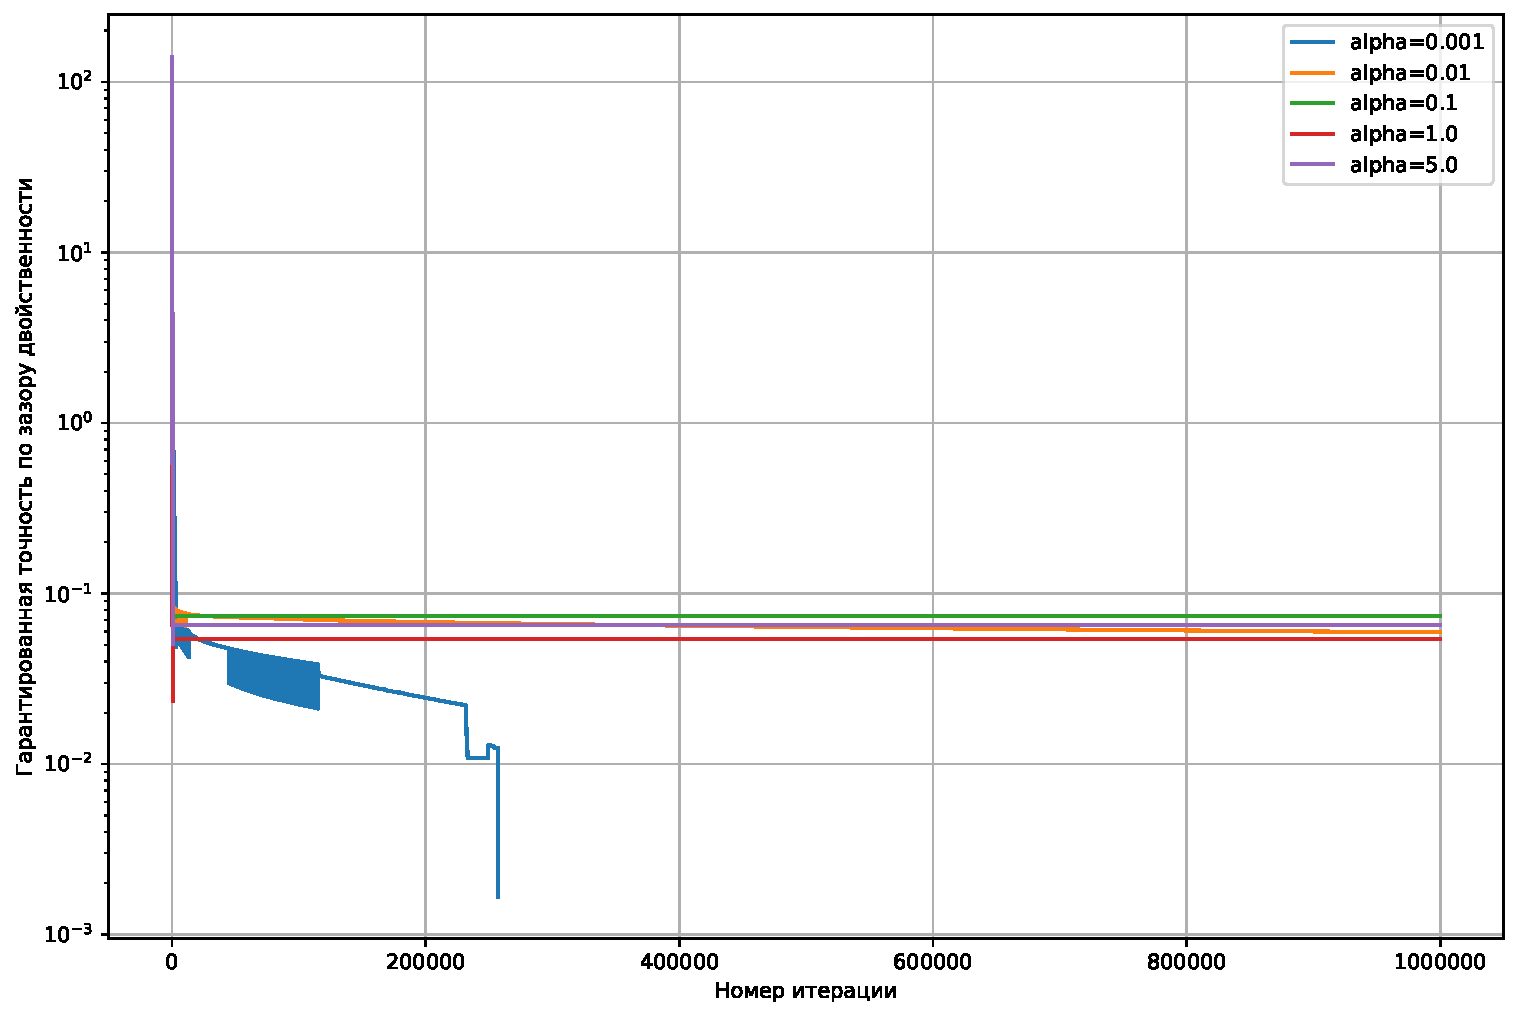
\includegraphics[width=.45\textwidth]{pics/1/subgradient_gap_vs_iter_alpha_x_0_bodyfat.pdf}
 		} &

		\subfloat{
    		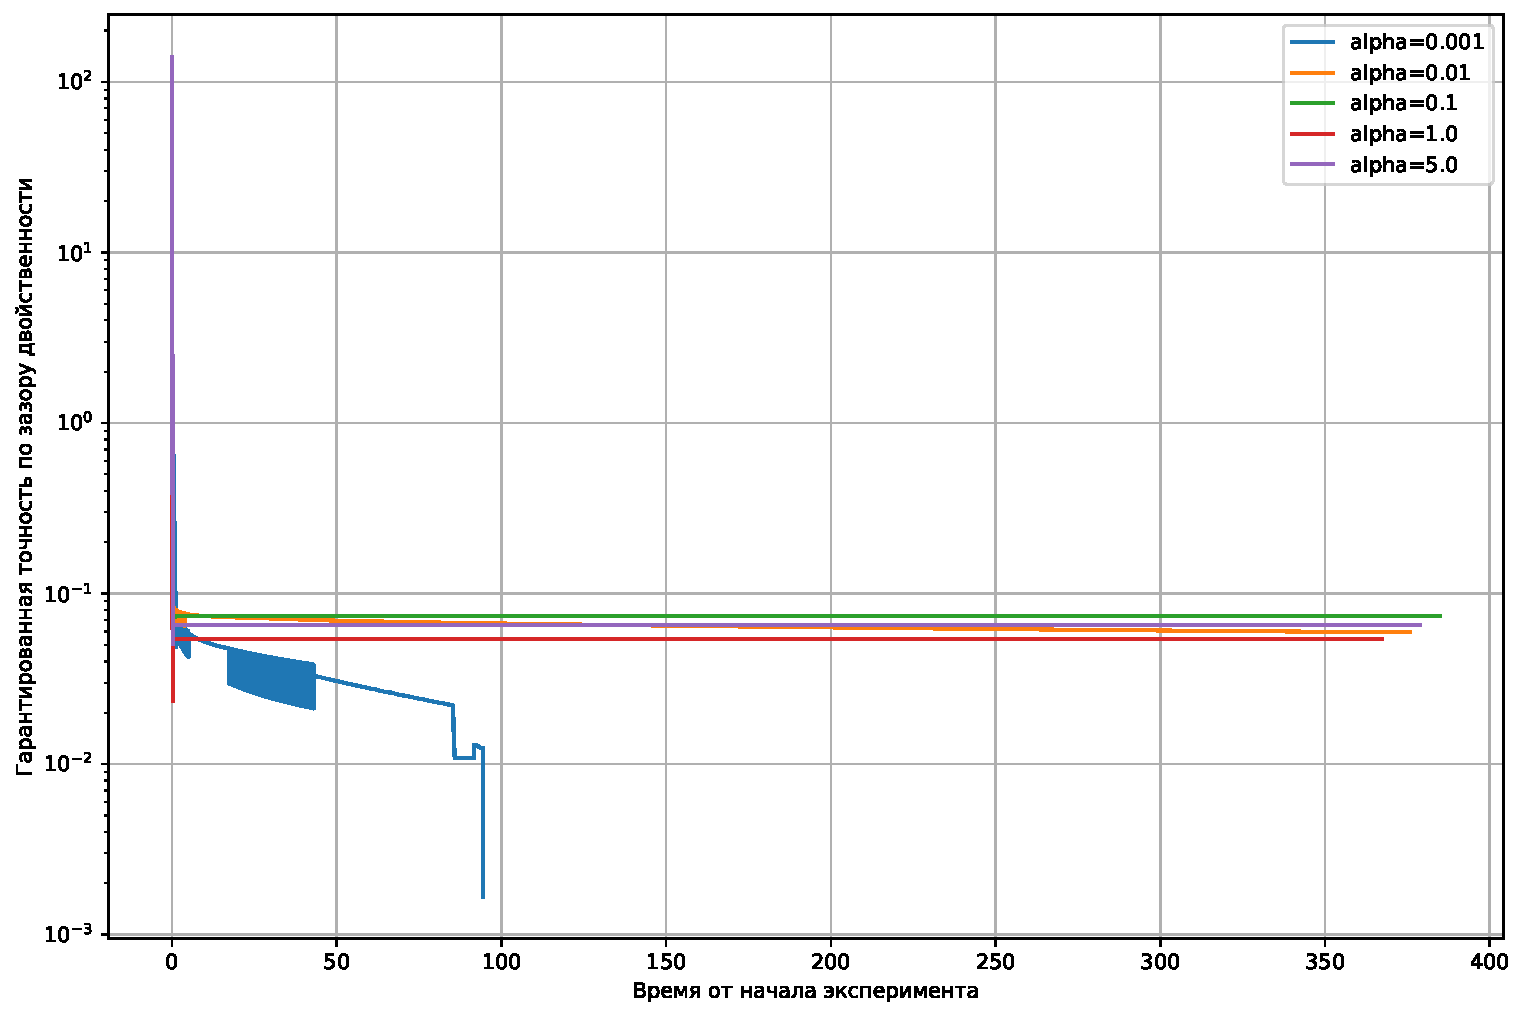
\includegraphics[width=.45\textwidth]{pics/1/subgradient_gap_vs_time_alpha_x_0_bodyfat.pdf}
 		}
   \end{tabular}
   \captionsetup{justification=centering}
   \caption{Поведение субградиентного метода при разных значениях $\alpha_0$ с начальной точкой $x_0 = 0_n$ на наборе данных bodyfat}
\end{figure}

\begin{figure}[H]
	\captionsetup{font=scriptsize}
	\centering
	\begin{tabular}[c]{cc}
		\subfloat{
    		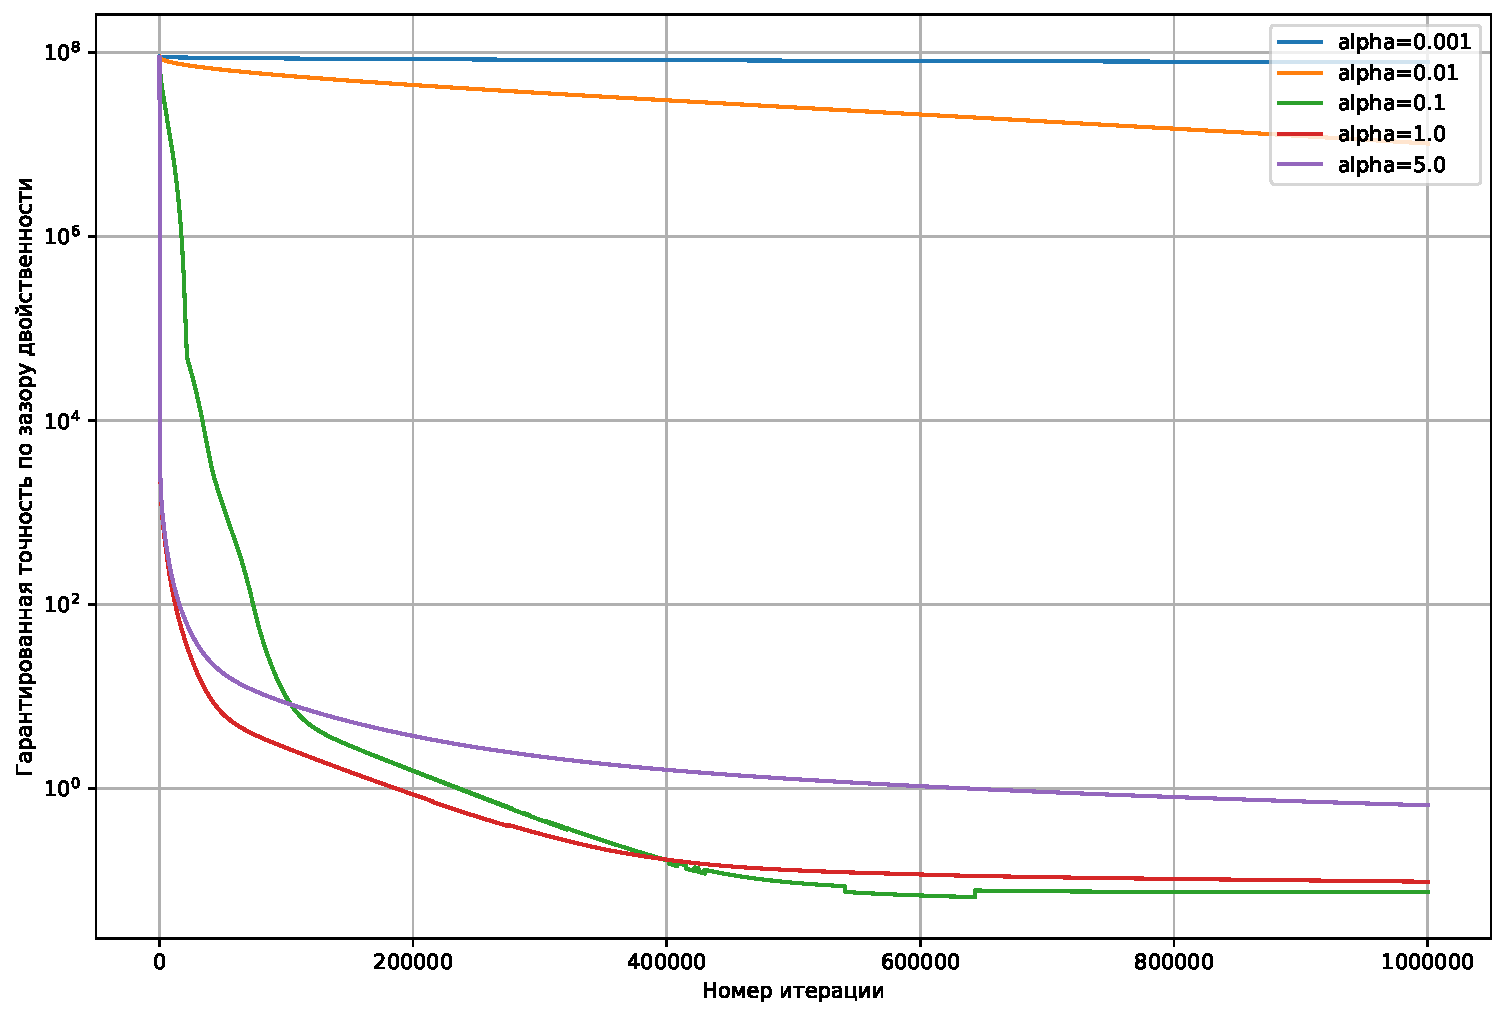
\includegraphics[width=.45\textwidth]{pics/1/subgradient_gap_vs_iter_alpha_x_1_bodyfat.pdf}
 		} &

		\subfloat{
    		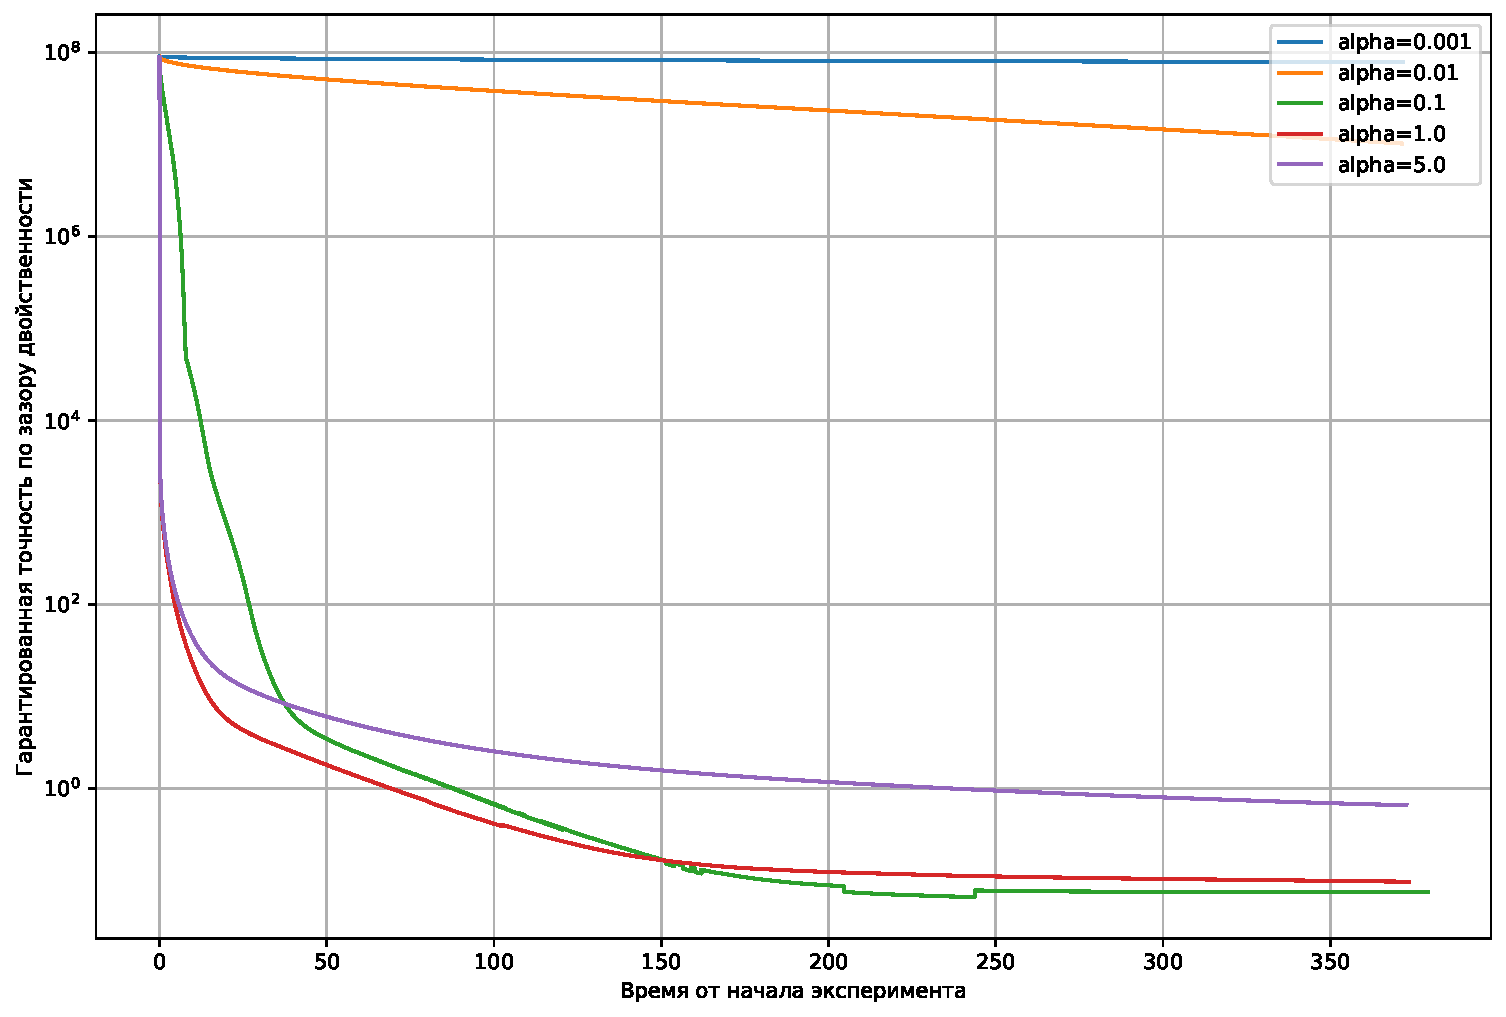
\includegraphics[width=.45\textwidth]{pics/1/subgradient_gap_vs_time_alpha_x_1_bodyfat.pdf}
 		}
   \end{tabular}
   \captionsetup{justification=centering}
   \caption{Поведение субградиентного метода при разных значениях $\alpha_0$ с начальной точкой $x_0 = 1_n$ на наборе данных bodyfat}
\end{figure}


\begin{figure}[H]
	\captionsetup{font=scriptsize}
	\centering
	\begin{tabular}[c]{cc}
		\subfloat{
    		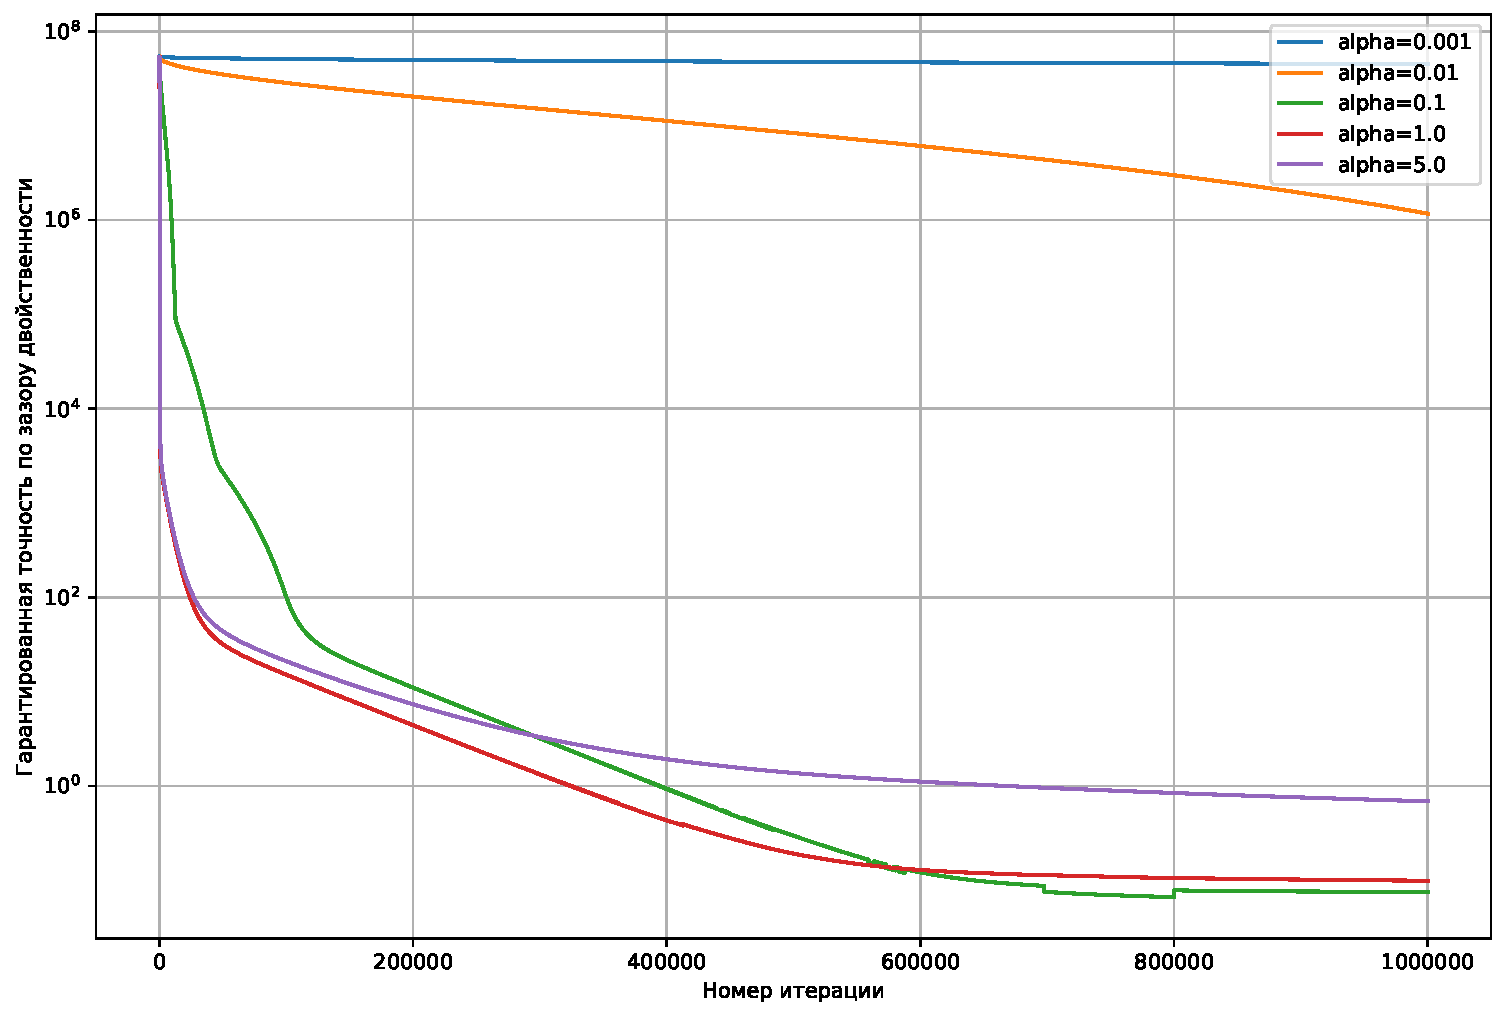
\includegraphics[width=.45\textwidth]{pics/1/subgradient_gap_vs_iter_alpha_x_2_bodyfat.pdf}
 		} &

		\subfloat{
    		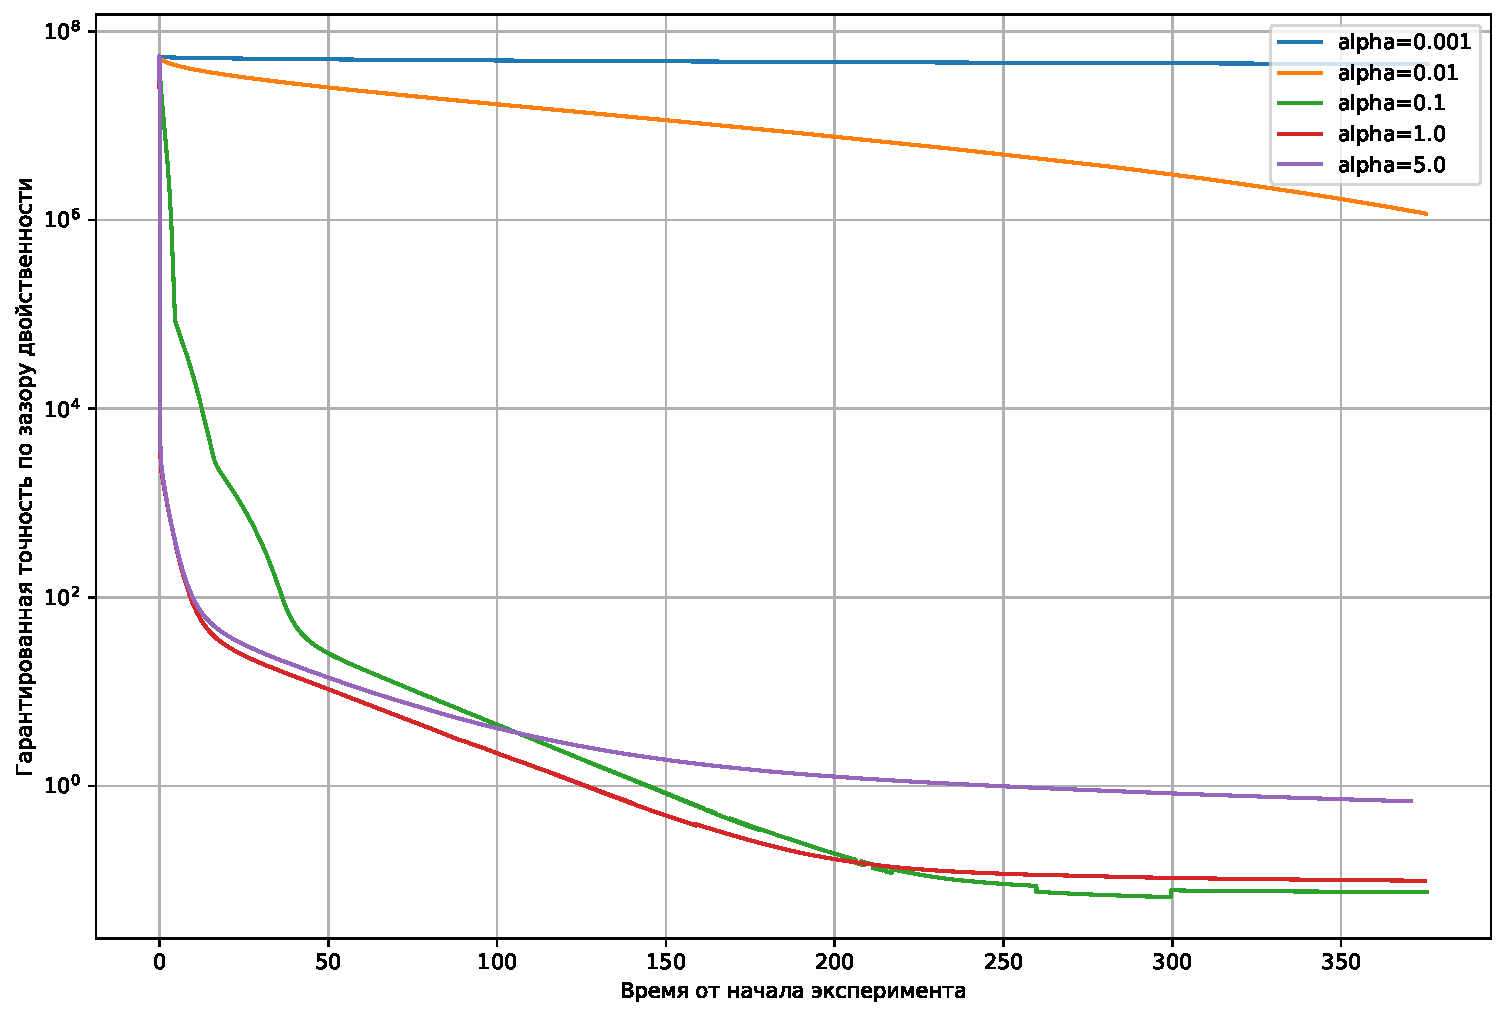
\includegraphics[width=.45\textwidth]{pics/1/subgradient_gap_vs_time_alpha_x_2_bodyfat.pdf}
 		}
   \end{tabular}
   \captionsetup{justification=centering}
   \caption{Поведение субградиентного метода при разных значениях $\alpha_0$ с начальной точкой $x_0 \sim N(0, I_n)$ на наборе данных bodyfat}
\end{figure}

Влияние выбора начальной точки явно видно: в случае $x_0 = 0_n$ мы наблюдаем единственный случай сходимости за весь эксперимент ($\alpha=0.001$), но при этом мы видим <<застревание>> метода при других значениях $\alpha_0$. Тем не менее, субградиентный метод всё равно достигает меньших значений зазора двойственности с $x_0$, чем с другими начальными точками. 

При значениях $\alpha_0 \geq 0.1$ на последних двух парах графиков мы имеем примерно одинаковые наблюдения, а при $\alpha_0 \leq 0.01$ зазор двойственности практически не уменьшается. 

Значение $alpha_0=0.001$ является одновременно и лучшим, и худшим при разном выборе начальной точке.
Поэтому можно предположить, что есть некоторая зависимость между длиной шага и начальной точкой.

\subsubsection{Набор данных housing}

\begin{figure}[H]
	\captionsetup{font=scriptsize}
	\centering
	\begin{tabular}[c]{cc}
		\subfloat{
    		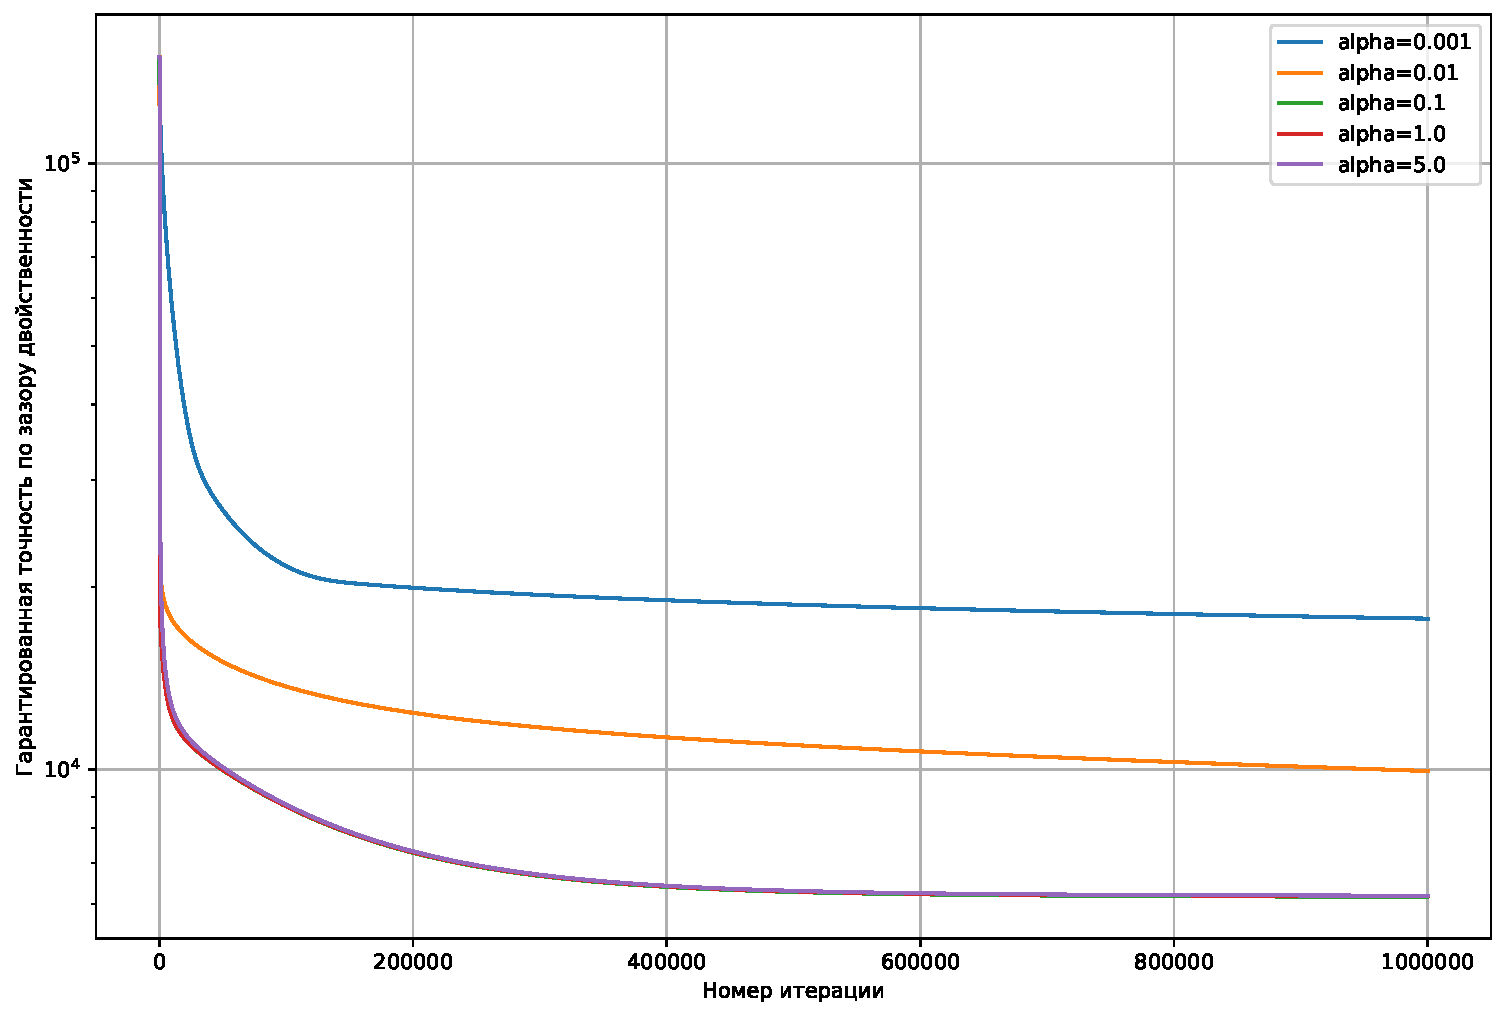
\includegraphics[width=.45\textwidth]{pics/1/subgradient_gap_vs_iter_alpha_x_0_housing.pdf}
 		} &

		\subfloat{
    		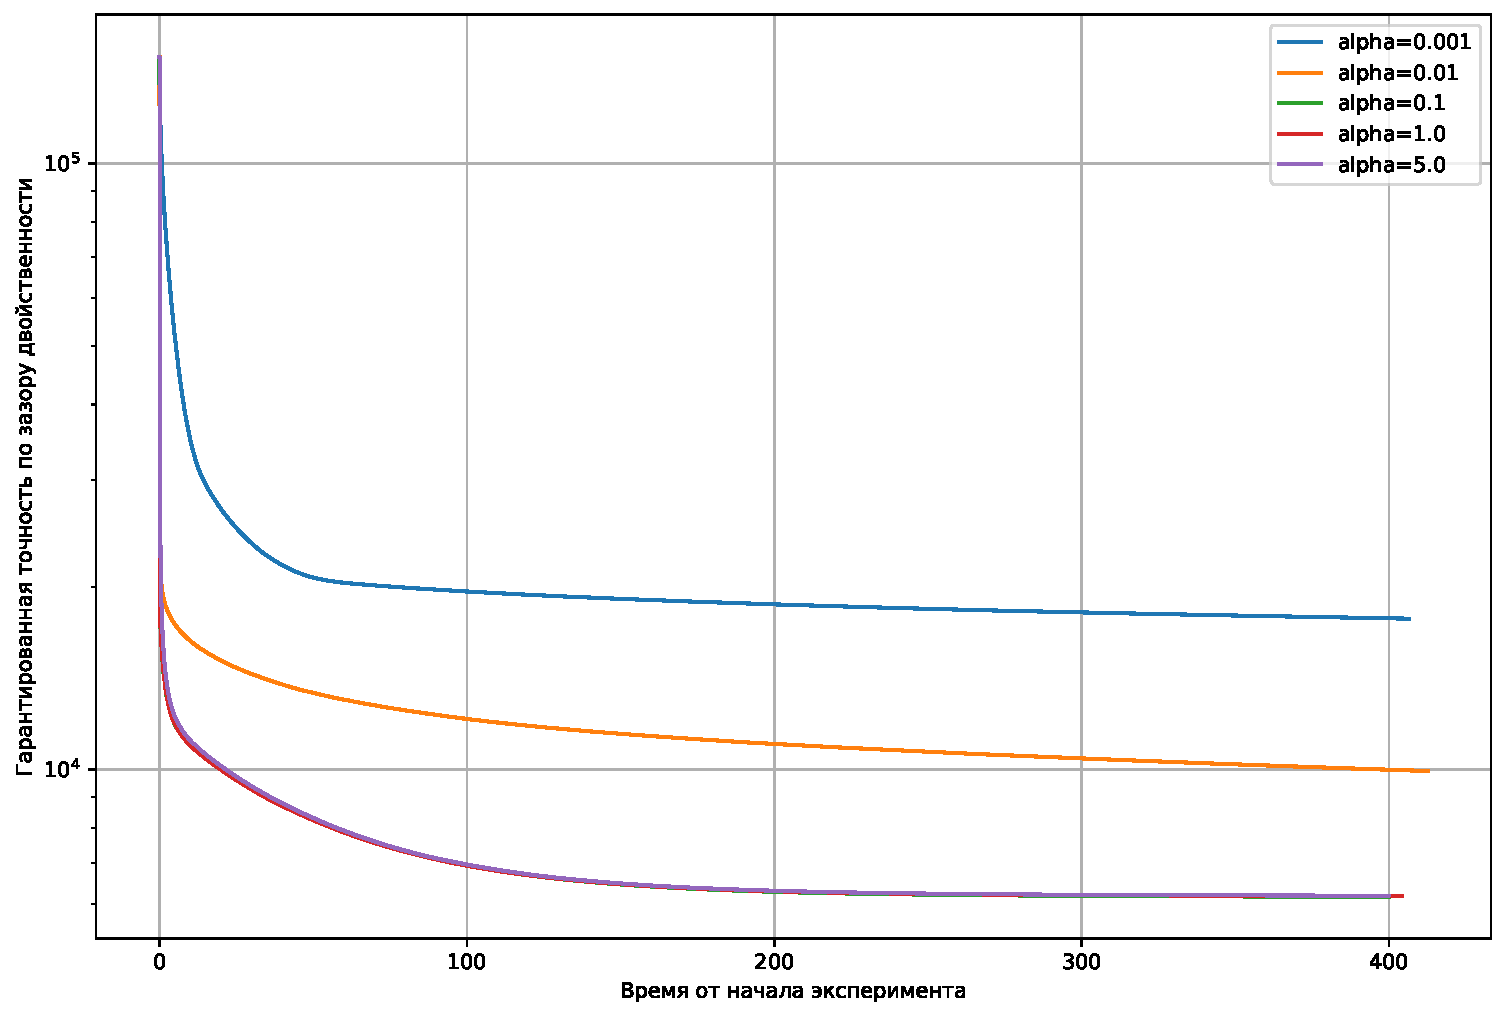
\includegraphics[width=.45\textwidth]{pics/1/subgradient_gap_vs_time_alpha_x_0_housing.pdf}
 		}
   \end{tabular}
   \captionsetup{justification=centering}
   \caption{Поведение субградиентного метода при разных значениях $\alpha_0$ с начальной точкой $x_0 = 0_n$ на наборе данных housing}
\end{figure}

\begin{figure}[H]
	\captionsetup{font=scriptsize}
	\centering
	\begin{tabular}[c]{cc}
		\subfloat{
    		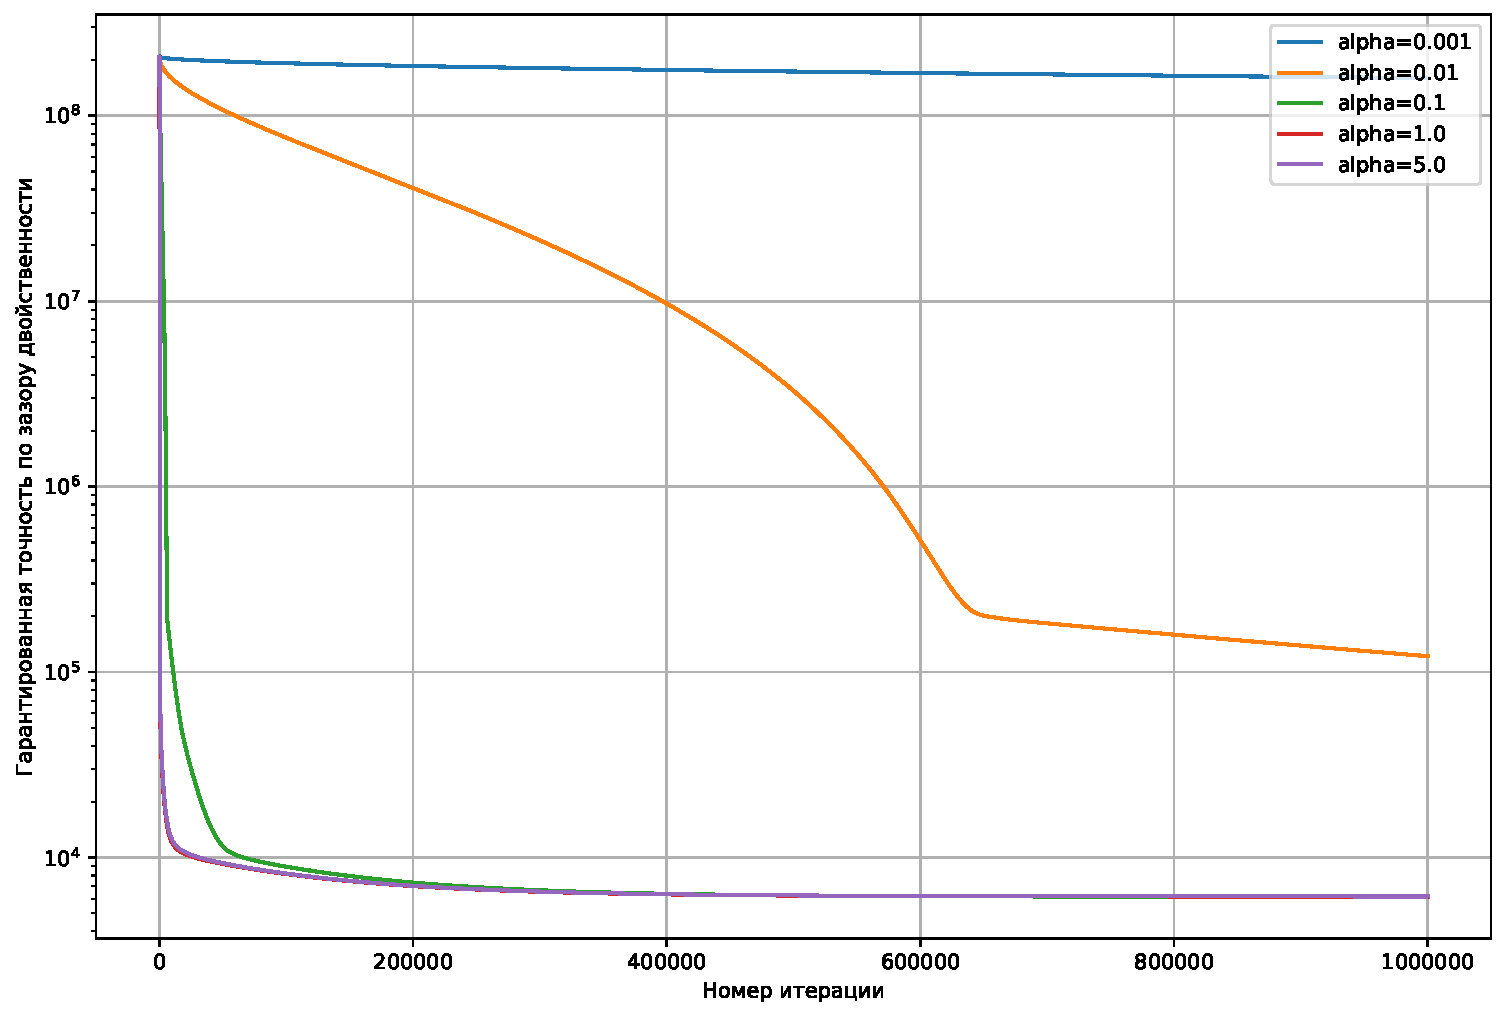
\includegraphics[width=.45\textwidth]{pics/1/subgradient_gap_vs_iter_alpha_x_1_housing.pdf}
 		} &

		\subfloat{
    		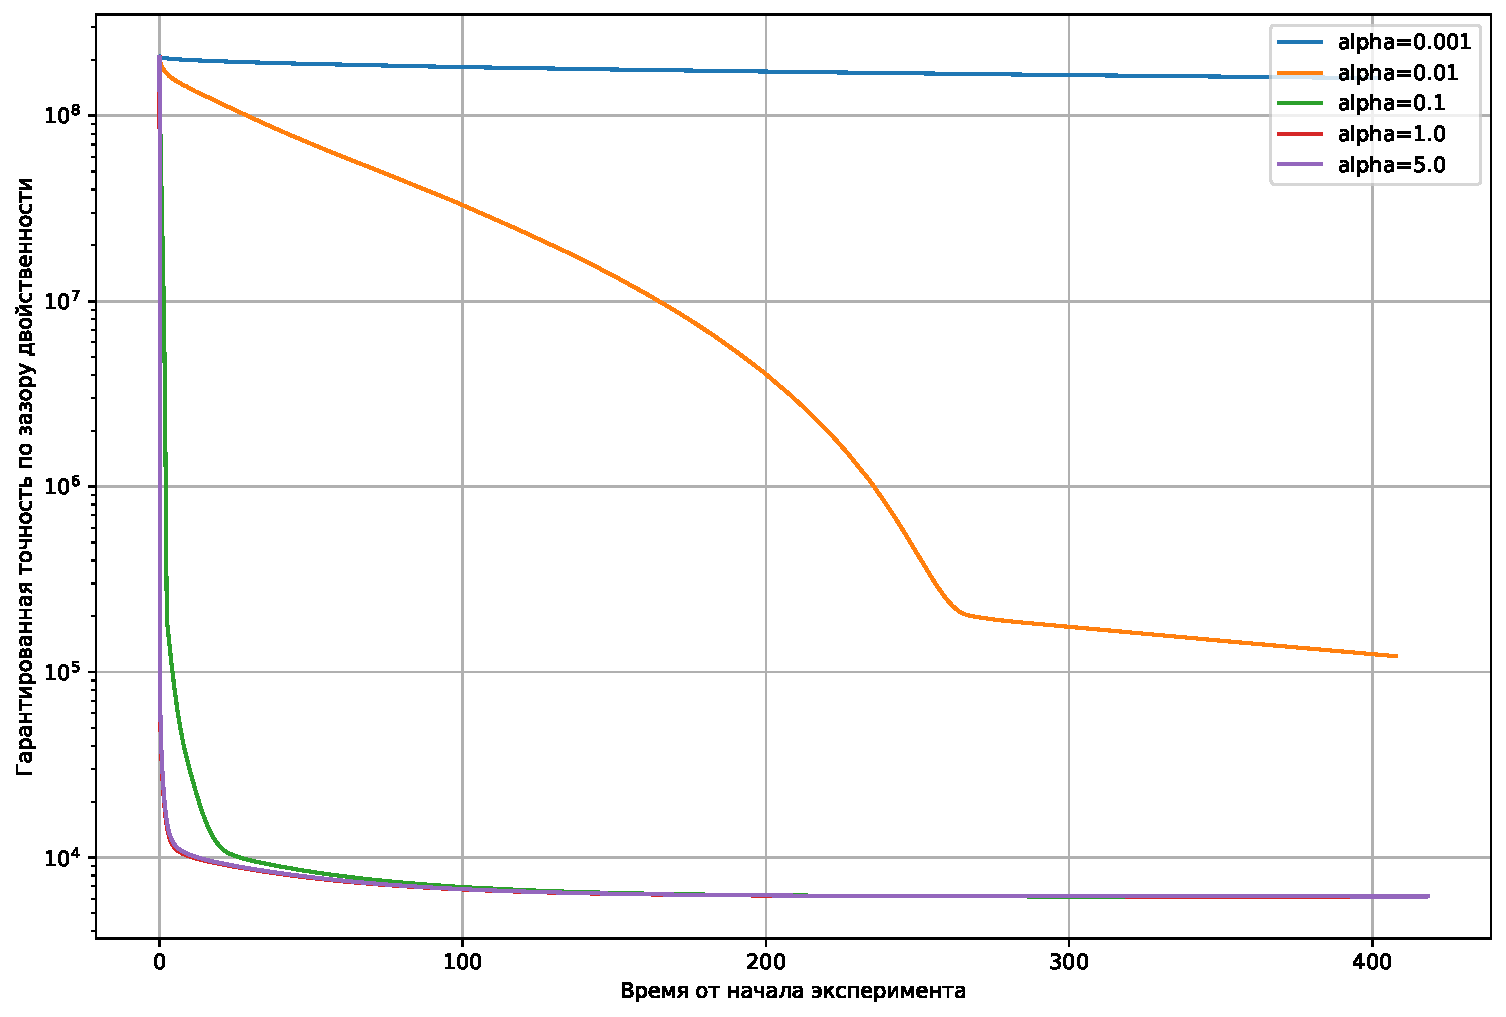
\includegraphics[width=.45\textwidth]{pics/1/subgradient_gap_vs_time_alpha_x_1_housing.pdf}
 		}
   \end{tabular}
   \captionsetup{justification=centering}
   \caption{Поведение субградиентного метода при разных значениях $\alpha_0$ с начальной точкой $x_0 = 1_n$ на наборе данных housing}
\end{figure}


\begin{figure}[H]
	\captionsetup{font=scriptsize}
	\centering
	\begin{tabular}[c]{cc}
		\subfloat{
    		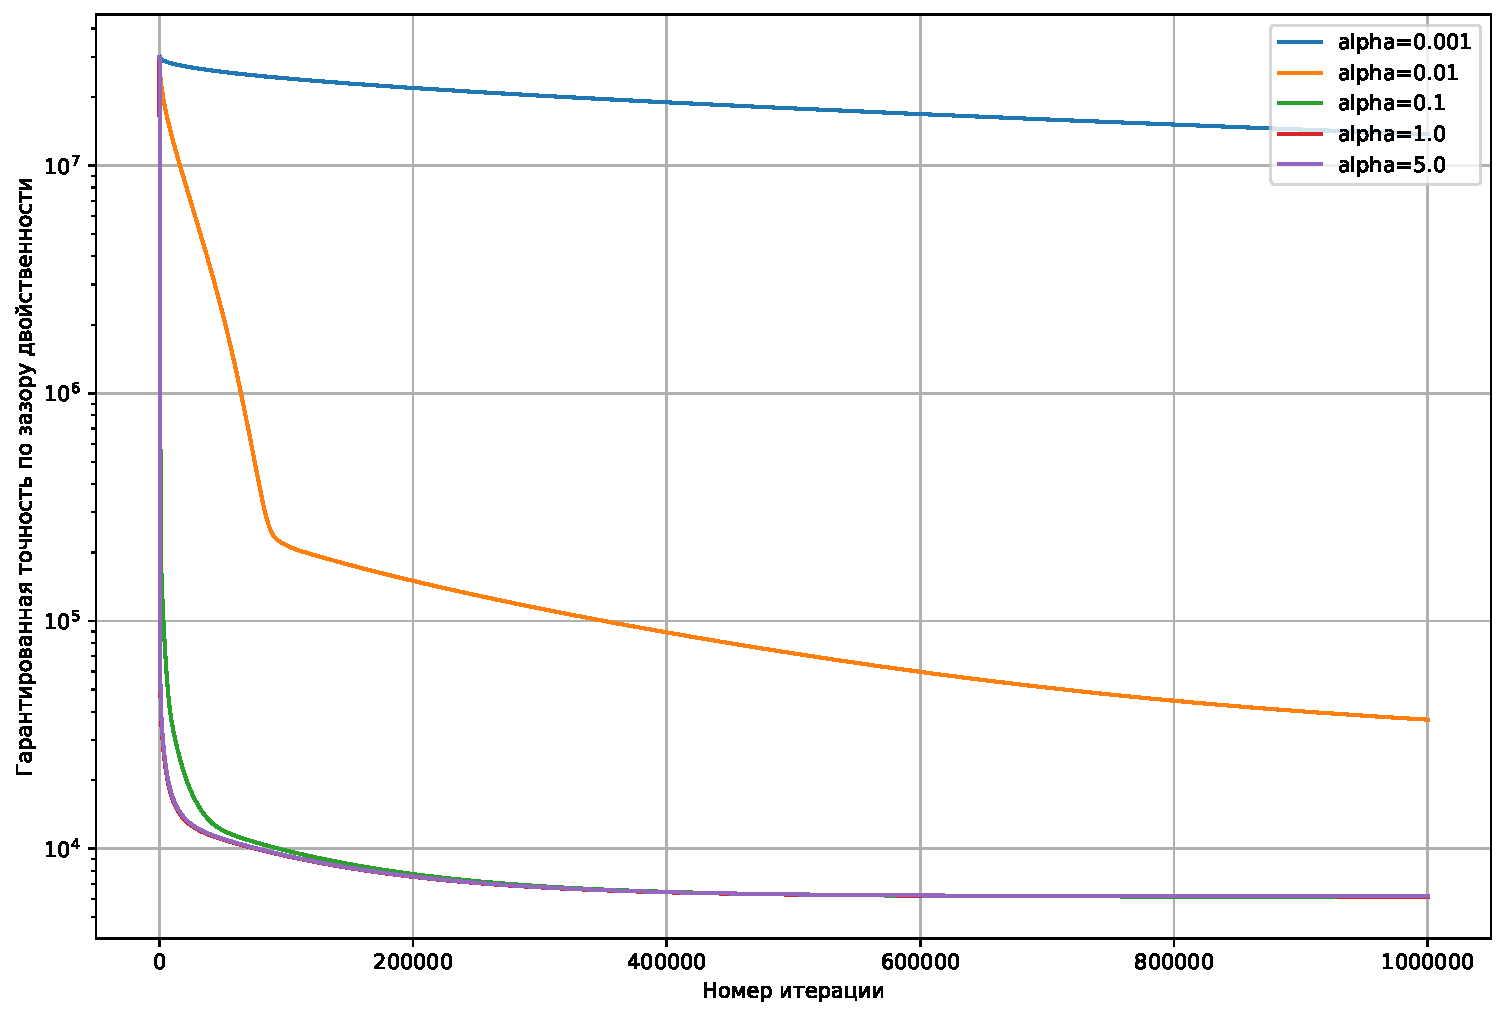
\includegraphics[width=.45\textwidth]{pics/1/subgradient_gap_vs_iter_alpha_x_2_housing.pdf}
 		} &

		\subfloat{
    		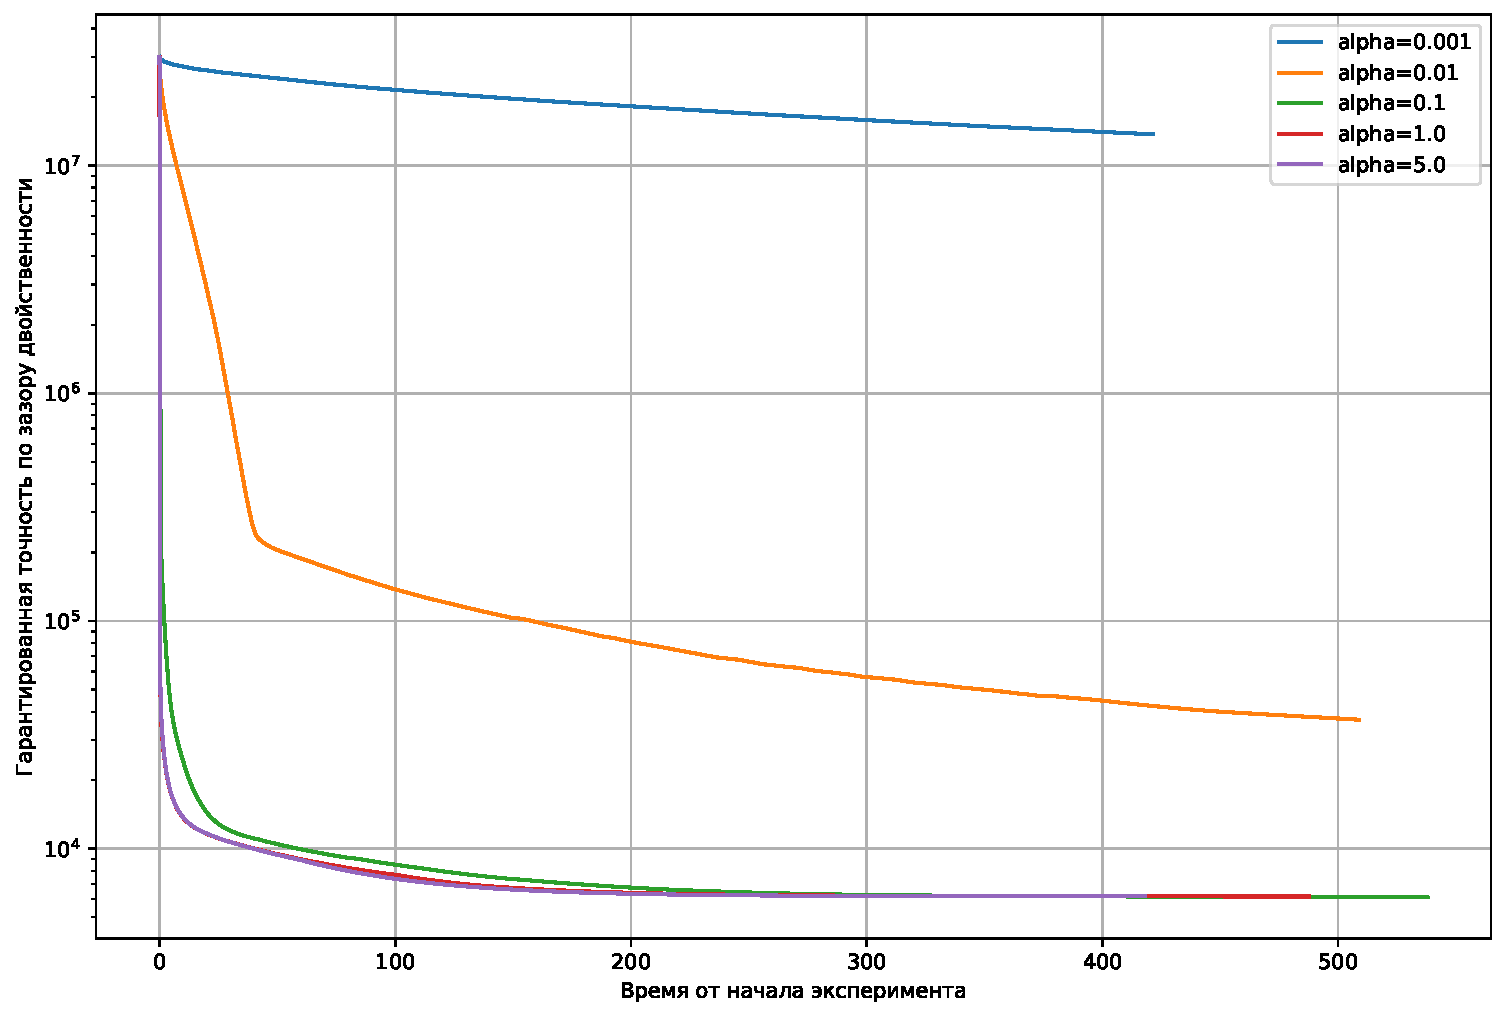
\includegraphics[width=.45\textwidth]{pics/1/subgradient_gap_vs_time_alpha_x_2_housing.pdf}
 		}
   \end{tabular}
   \captionsetup{justification=centering}
   \caption{Поведение субградиентного метода при разных значениях $\alpha_0$ с начальной точкой $x_0 \sim N(0, I_n)$ на наборе данных housing}
\end{figure}

При $\alpha \geq 0.1$ кривые сливаются в одну кривую, находящуюся существенно ниже остальных.
На этот раз точка $x_0 = 0_n$ оказалась наоборот самой неудачной.
Здесь не прослеживается связь между выбором начальной точки и начальной длиной шага, но выбор начальной точки существенно влияет на работу субградиентного метода сам по себе.

В целом, кажется, что хорошим выбором для начальной длины шага будут значения порядка $10^{-1}$ или $10^0$, но, как мы видели на примере предыдущего набора данных, могут быть и исключения.

\subsubsection{Среднее число итераций одномерного поиска в градиентных методах}

Проверим, действительно ли число итераций одномерного поиска для подбора $L$ в проксимальных градиентных методах примерно равно 2. Построим графики суммарного числа итераций одномерного поиска для стандартной версии алгоритма и для его ускоренной версии на наборах данных housing и bodyfat.
Максмальное число итераций равно 10000.

\begin{figure}[H]
	\captionsetup{font=scriptsize}
	\centering
	\begin{tabular}[c]{cc}
		\subfloat[Набор данных bodyfat]{
    		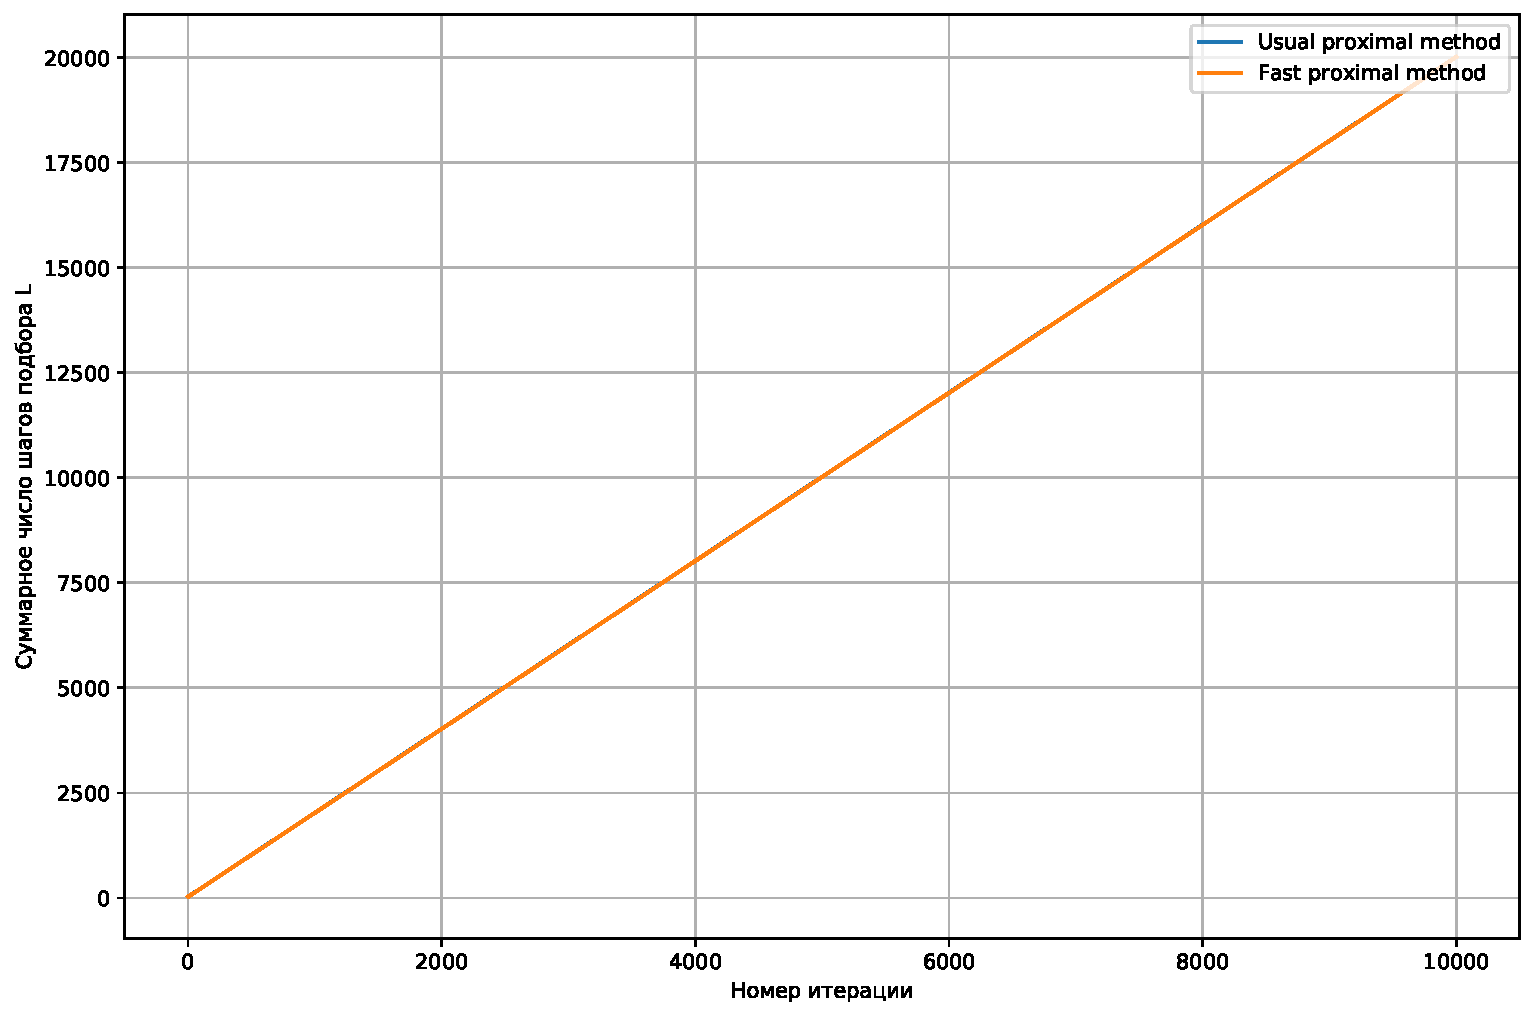
\includegraphics[width=.45\textwidth]{pics/2/prox_methods_steps_bodyfat.pdf}
 		}
 		
 		&

		\subfloat[Набор данных housing]{
    		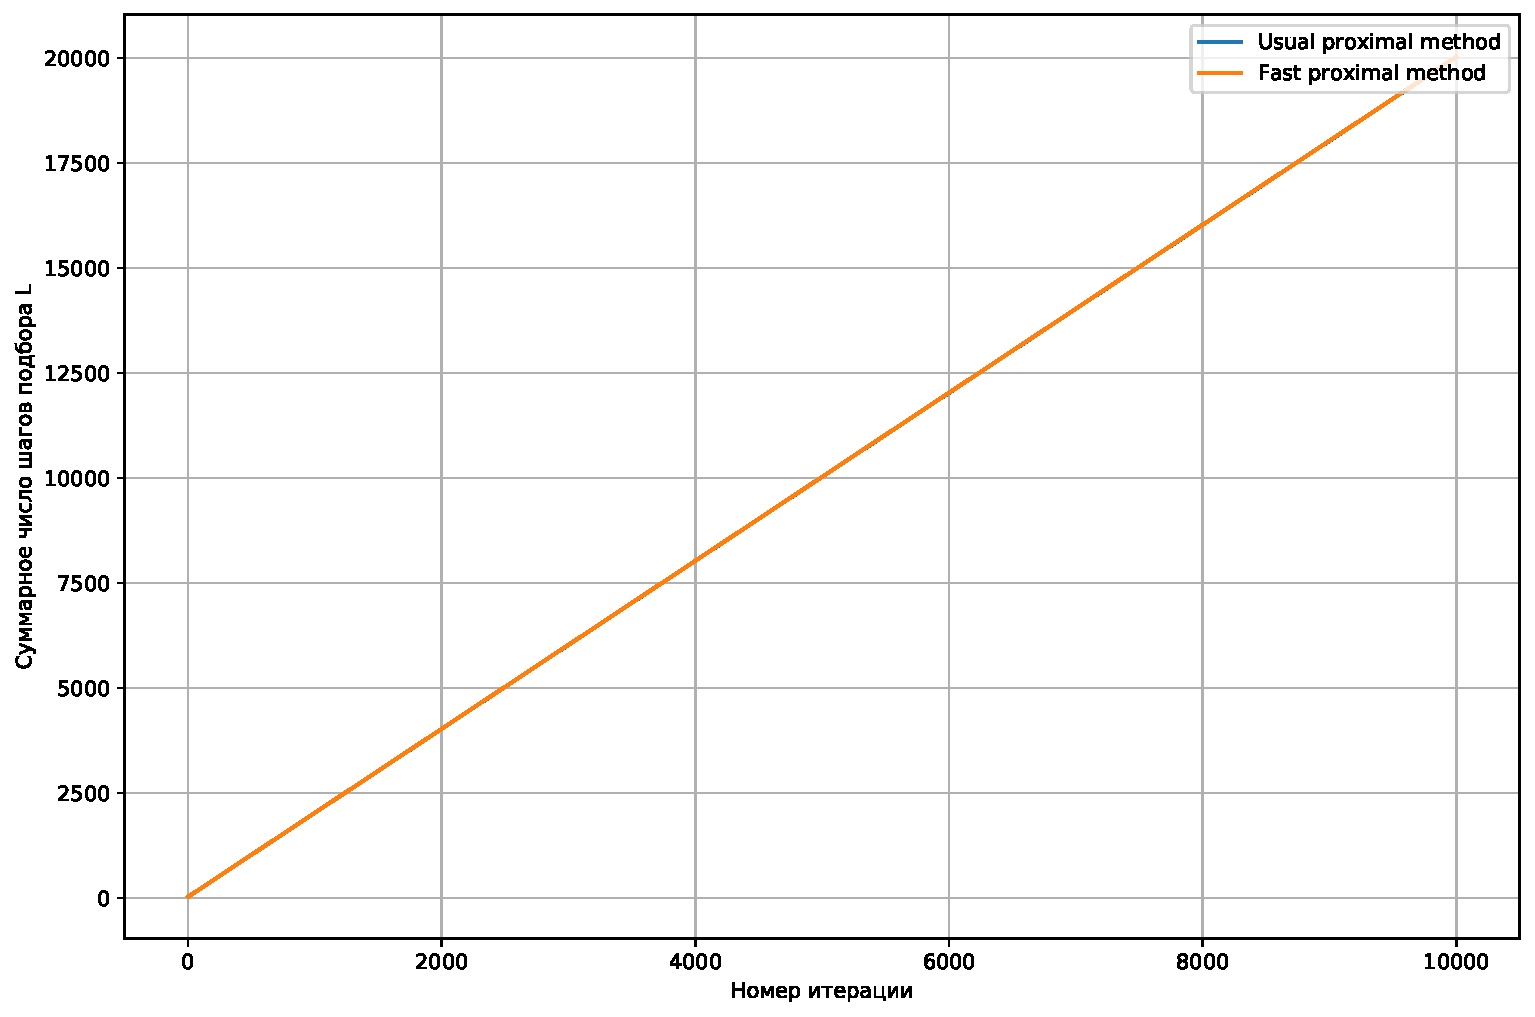
\includegraphics[width=.45\textwidth]{pics/2/prox_methods_steps_housing.pdf}
 		}
   \end{tabular}
   \captionsetup{justification=centering}
   \caption{Суммарное число итераций одномерного поиска для градиентных методов}
\end{figure}

Графики для обеих версий градиентного метода неразличимы на вид. На обоих наборах данных наблюдается одинаковая картина. Видно, что кривые на графиках выглядят как прямая с коэффициентом наклона равным 2.
Это подтверждает, что в среднем делается примерно две итерации одномерного поиска.

\subsection{Зависимость работы методов от размерности пространства $n$, размера выборки $m$ и коэффициентра регуляризации $\lambda$}

	Будем генерировать компоненты матрицы объектов-признаков и целевого вектора из стандартного нормального распределения.

За начальную точку возьмём $x_0 = 0$.

Положим $m=100$, $n=100$, $\lambda=1.0$ как стандартные значения параметров.
Будем изменять каждый из них в отдельности и брать оставшиеся равными стандартным значениям.

\subsubsection{Зависимость от $n$}
\begin{figure}[H]
	\captionsetup{font=scriptsize}
	\centering
	\begin{tabular}[c]{ccc}
		\subfloat[субградиентный метод]{
    		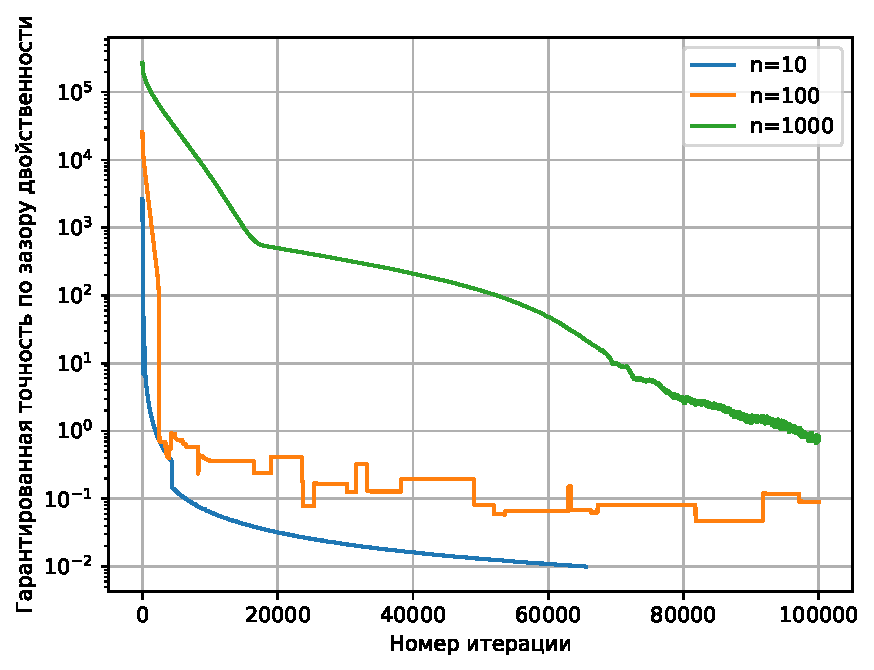
\includegraphics[width=.3\textwidth]{pics/3/subgradient/lasso_gap_vs_iter_n.pdf}
 		} &

		\subfloat[градиентный методы]{
    		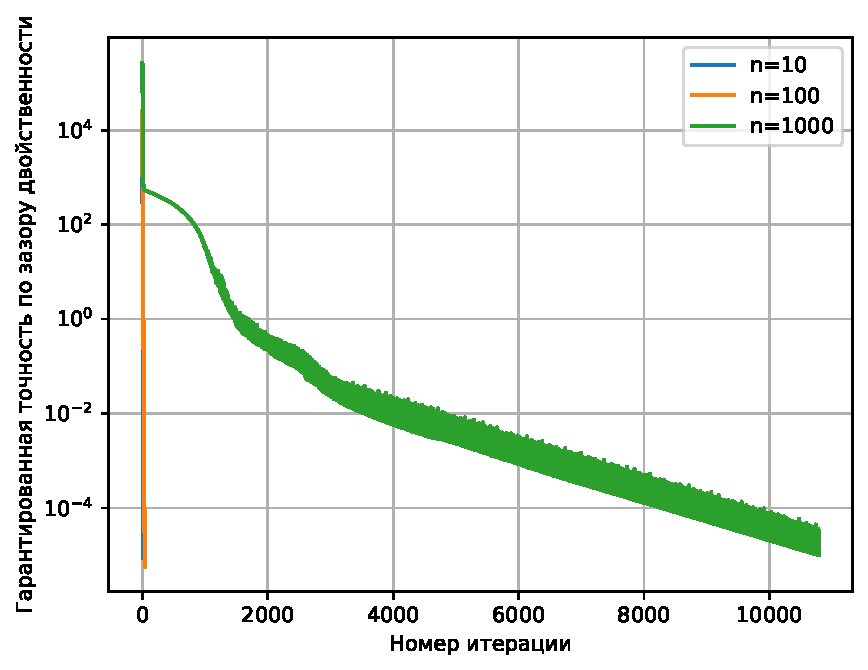
\includegraphics[width=.3\textwidth]{pics/3/proximal/lasso_gap_vs_iter_n.pdf}
 		} &
 		
 		\subfloat[уск. градиентный метод]{
    		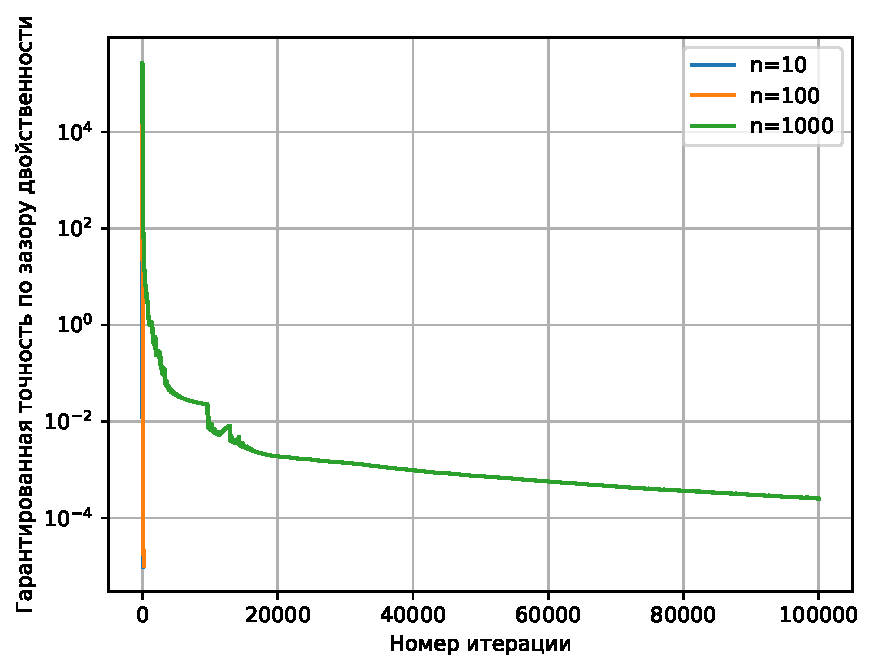
\includegraphics[width=.3\textwidth]{pics/3/proximal_fast/lasso_gap_vs_iter_n.pdf}
 		}

   \end{tabular}
   \captionsetup{justification=centering}
   \caption{Гарантированная точность по зазору двойственности в зависимости от итерации при разных $n$ }
\end{figure}

\begin{figure}[H]
	\captionsetup{font=scriptsize}
	\centering
	\begin{tabular}[c]{ccc}
		\subfloat[субградиентный метод]{
    		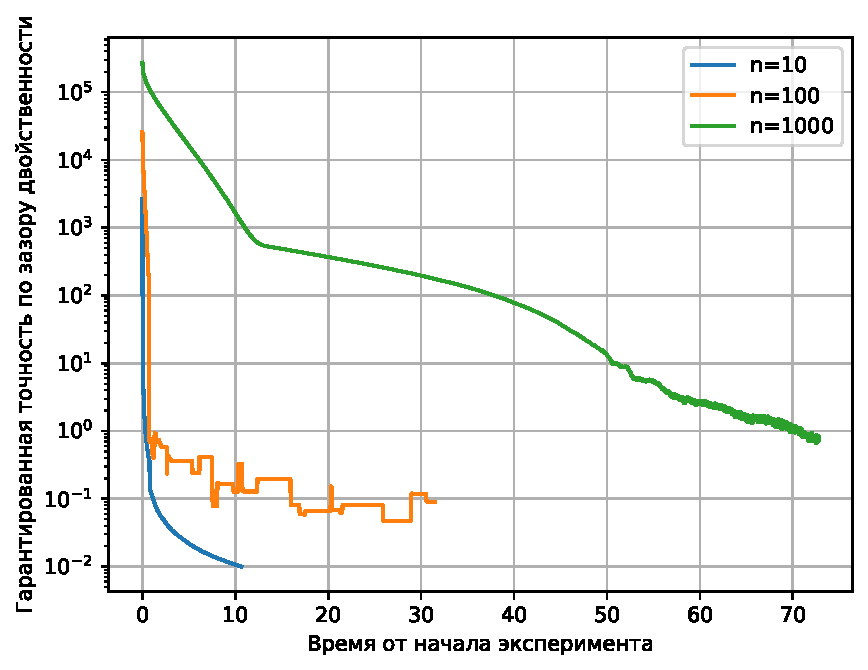
\includegraphics[width=.3\textwidth]{pics/3/subgradient/lasso_gap_vs_time_n.pdf}
 		} &

		\subfloat[градиентный метод]{
    		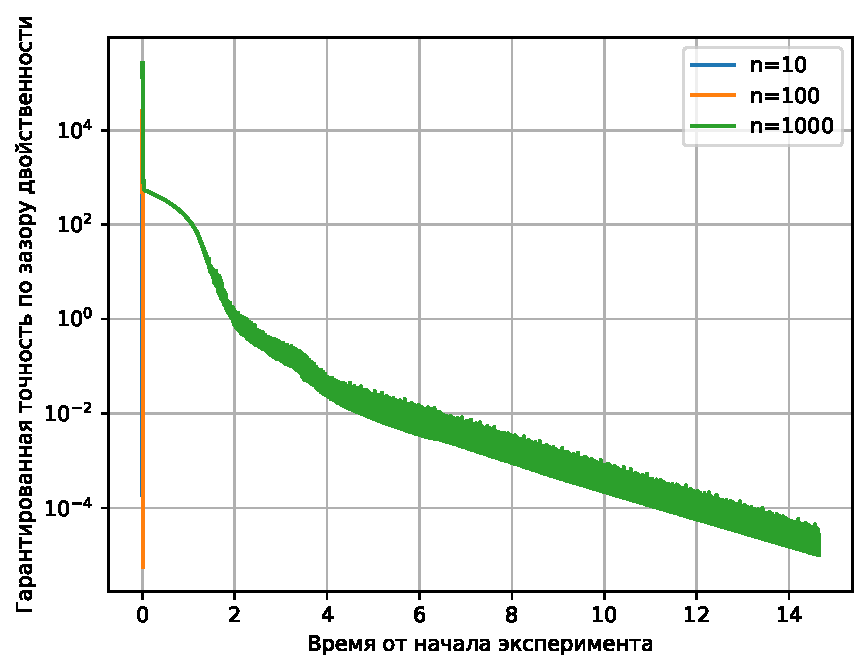
\includegraphics[width=.3\textwidth]{pics/3/proximal/lasso_gap_vs_time_n.pdf}
 		} &
 		
 		\subfloat[уск. градиентный метод]{
    		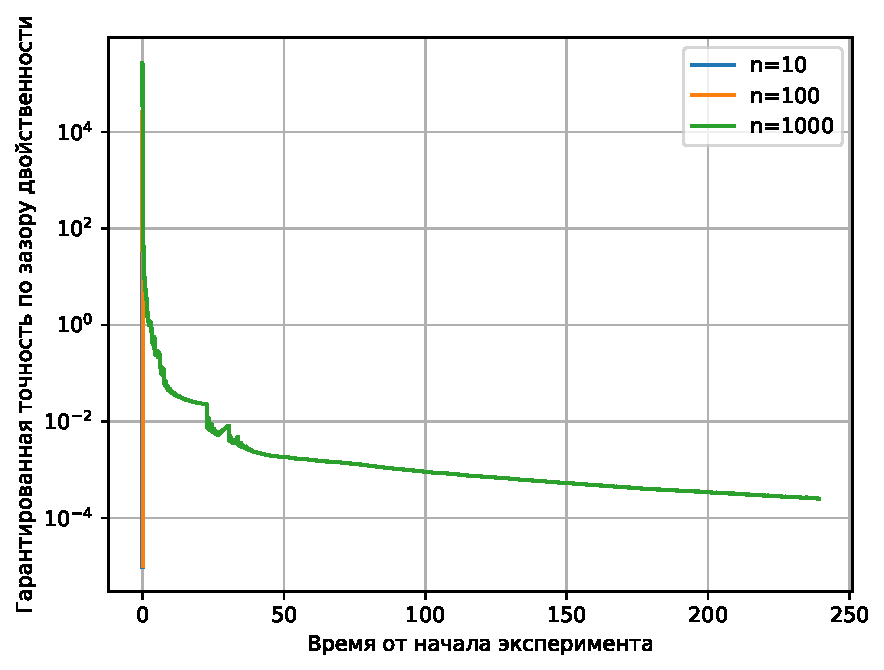
\includegraphics[width=.3\textwidth]{pics/3/proximal_fast/lasso_gap_vs_time_n.pdf}
 		}
   \end{tabular}
   \captionsetup{justification=centering}
   \caption{Гарантированная точность по зазору двойственности в зависимости от времени при разных $n$ }
\end{figure}

Видно, что градиентные методы работают существенно быстрее, чем субградиентный метод, как и ожидается.
Как ни странно, ускоренный метод сходится существенно медленнее (обратите внимание, что шкала абсцисс для градиентного метода оканчивается районе 10500 итераций). 
 
Как и ожидается, чем больше $n$, тем больше итераций и времени требуется алгоритмам.

\subsubsection{Зависимость от $m$}
\begin{figure}[H]
	\captionsetup{font=scriptsize}
	\centering
	\begin{tabular}[c]{ccc}
		\subfloat[субградиентный метод]{
    		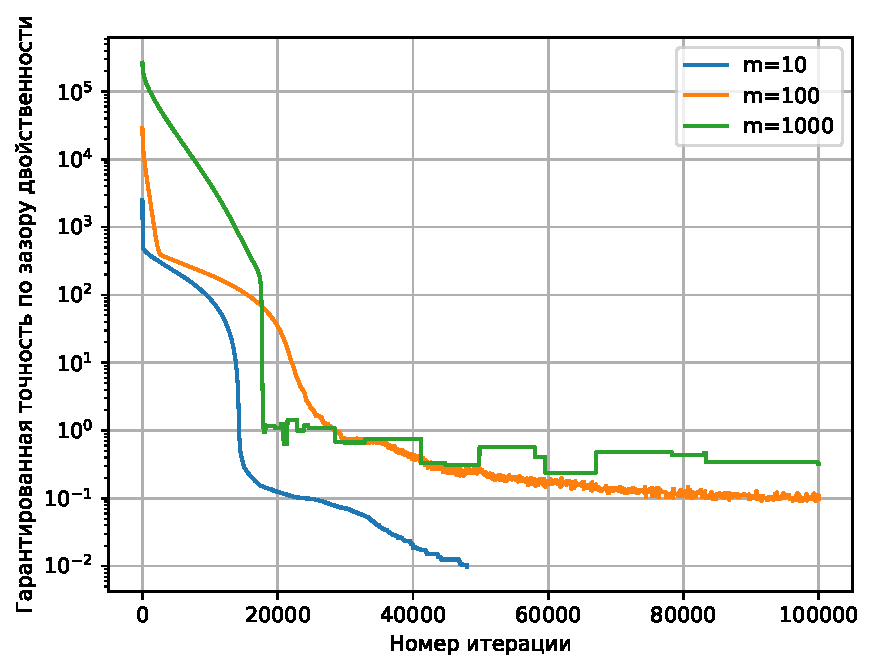
\includegraphics[width=.3\textwidth]{pics/3/subgradient/lasso_gap_vs_iter_m.pdf}
 		} &

		\subfloat[градиентный метод]{
    		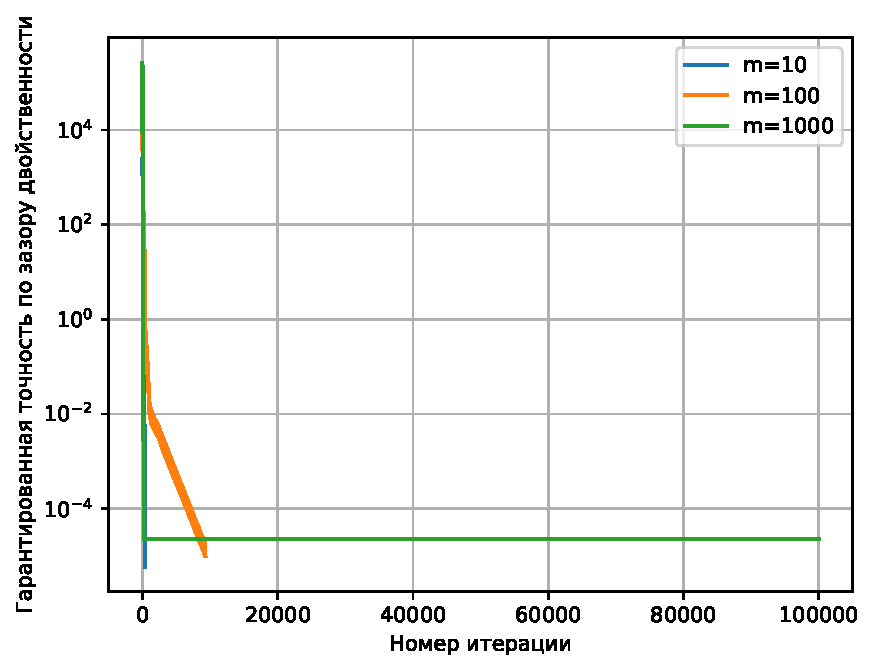
\includegraphics[width=.3\textwidth]{pics/3/proximal/lasso_gap_vs_iter_m.pdf}
 		} &
 		
 		\subfloat[уск. градиентный метод]{
    		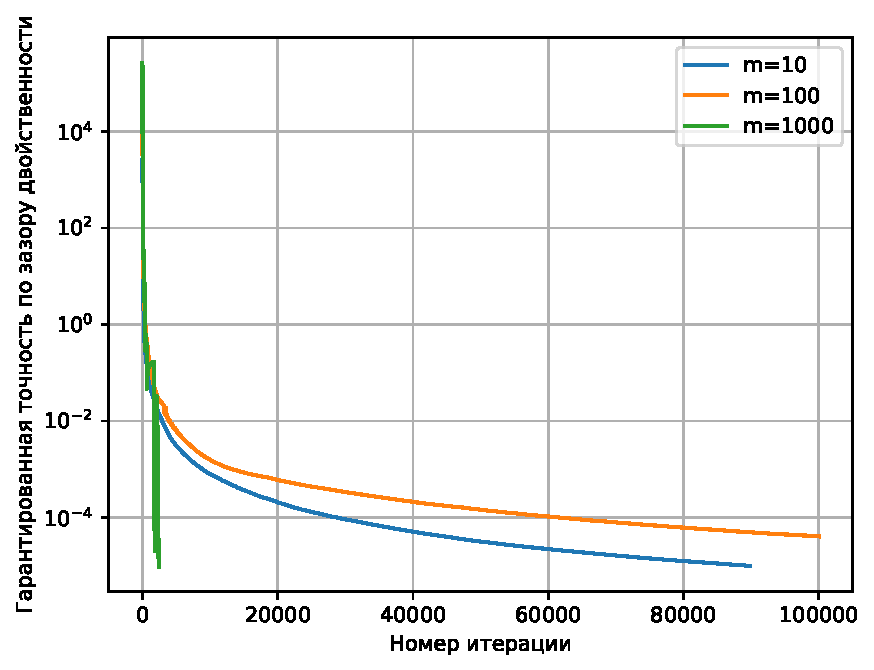
\includegraphics[width=.3\textwidth]{pics/3/proximal_fast/lasso_gap_vs_iter_m.pdf}
 		}

   \end{tabular}
   \captionsetup{justification=centering}
   \caption{Гарантированная точность по зазору двойственности в зависимости от итерации при разных $m$ }
\end{figure}

\begin{figure}[H]
	\captionsetup{font=scriptsize}
	\centering
	\begin{tabular}[c]{ccc}
		\subfloat[субградиентный метод]{
    		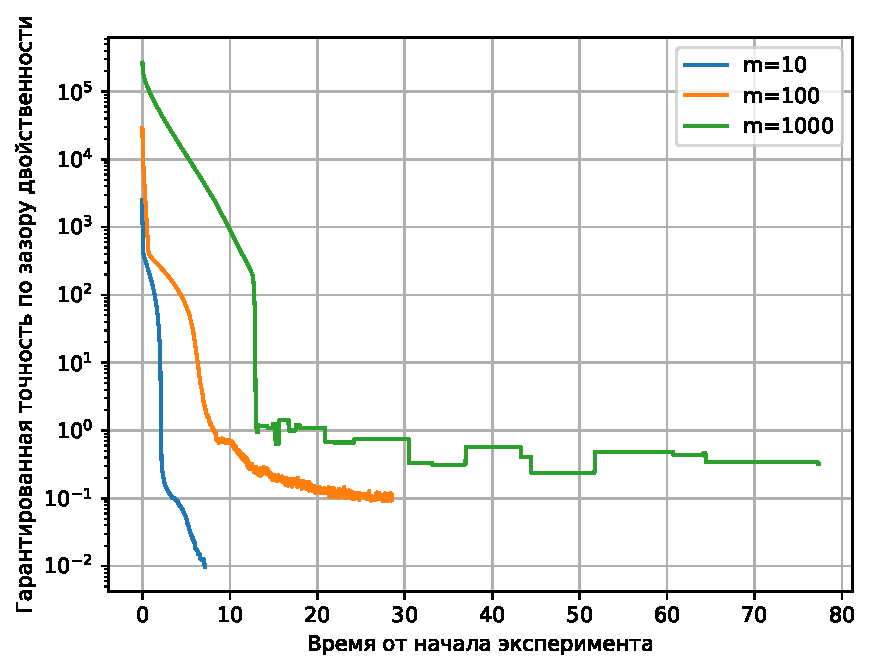
\includegraphics[width=.3\textwidth]{pics/3/subgradient/lasso_gap_vs_time_m.pdf}
 		} &

		\subfloat[градиентный метод]{
    		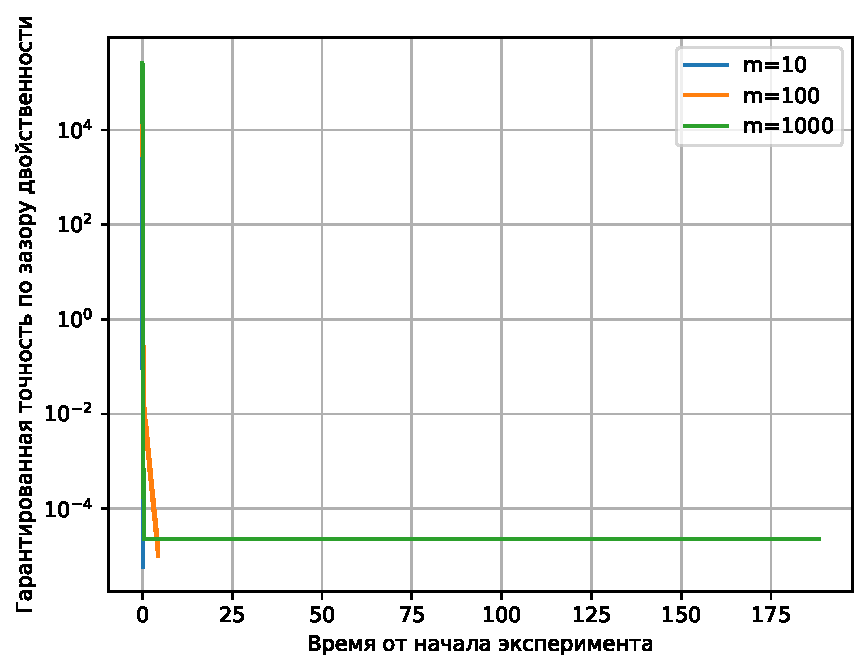
\includegraphics[width=.3\textwidth]{pics/3/proximal/lasso_gap_vs_time_m.pdf}
 		} &
 		
 		\subfloat[уск. градиентный метод]{
    		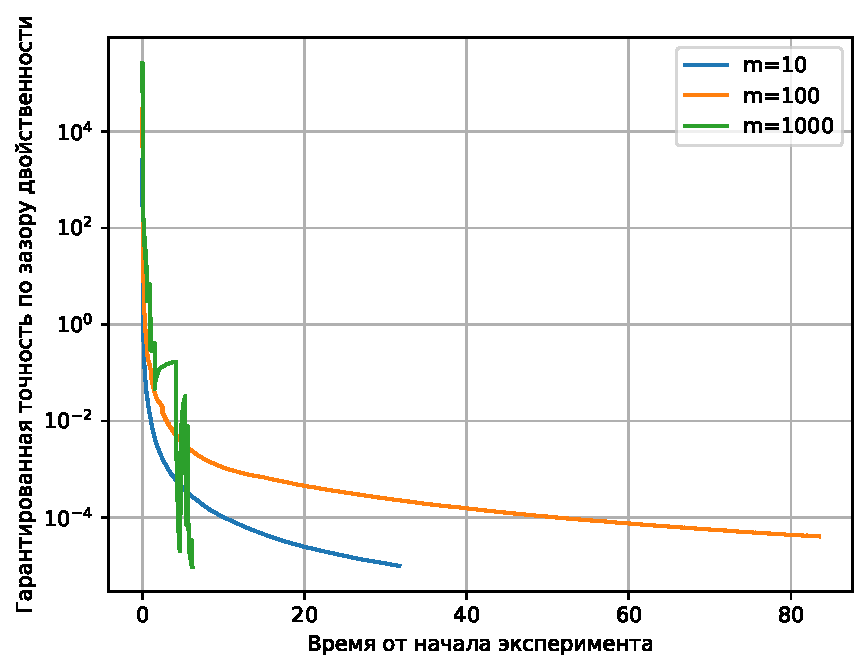
\includegraphics[width=.3\textwidth]{pics/3/proximal_fast/lasso_gap_vs_time_m.pdf}
 		}
   \end{tabular}
   \captionsetup{justification=centering}
   \caption{Гарантированная точность по зазору двойственности в зависимости от времени при разных $m$ }
\end{figure}

Здесь мы видим довольно неоднозначные результаты. 
В целом, градиентные методы справились лучше субградиентного.
При этом градиентный метод по какой-то причине застрял на некотором значении зазора двойственности при  $m =1000$, а ускоренная версия достигла довольно быстрой сходимости.
При этом при $m = 100$ ускоренный градиентный метод не сошелся в отличии от обычного градиентного метода, а при $m = 10$ сошелся гораздо позже.

Однозначный рост числа требуемых итераций  для достижения определенного значения зазора двойственности виден только для субградиентного метода.

\subsubsection{Зависимость от $\lambda$}

\begin{figure}[H]
	\captionsetup{font=scriptsize}
	\centering
	\begin{tabular}[c]{ccc}
		\subfloat[субградиентный метод]{
    		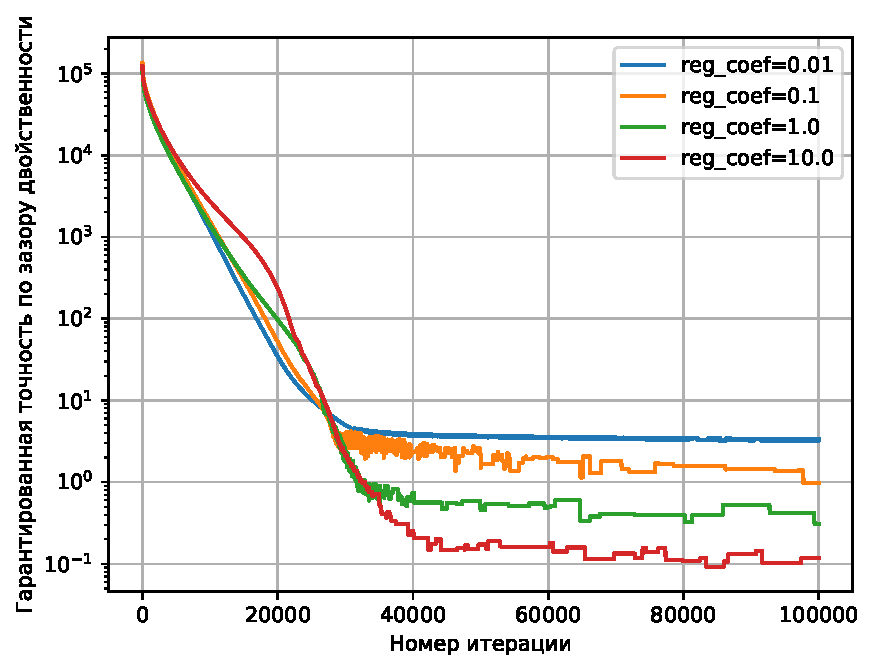
\includegraphics[width=.3\textwidth]{pics/3/subgradient/lasso_gap_vs_iter_reg_coef.pdf}
 		} &

		\subfloat[градиентный метод]{
    		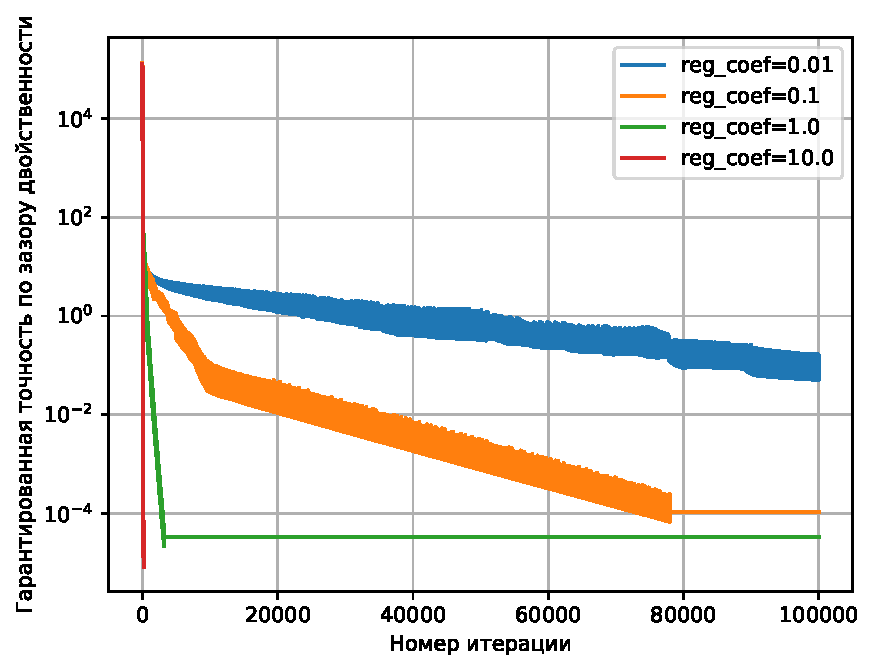
\includegraphics[width=.3\textwidth]{pics/3/proximal/lasso_gap_vs_iter_reg_coef.pdf}
 		} &
 		
 		\subfloat[уск. градиентный метод]{
    		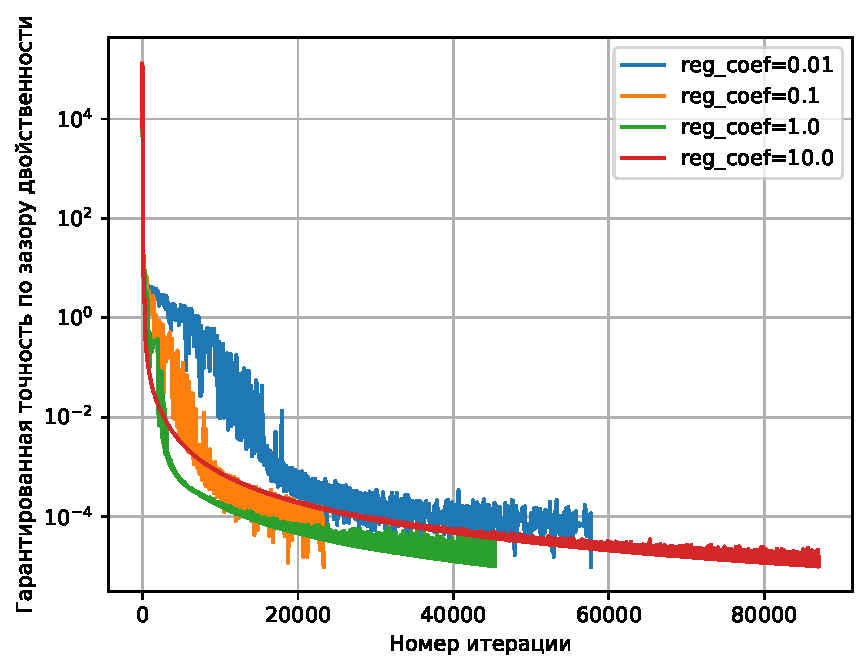
\includegraphics[width=.3\textwidth]{pics/3/proximal_fast/lasso_gap_vs_iter_reg_coef.pdf}
 		}

   \end{tabular}
   \captionsetup{justification=centering}
   \caption{Гарантированная точность по зазору двойственности в зависимости от итерации при разных $\lambda$ }
\end{figure}

\begin{figure}[H]
	\captionsetup{font=scriptsize}
	\centering
	\begin{tabular}[c]{ccc}
		\subfloat[субградиентный метод]{
    		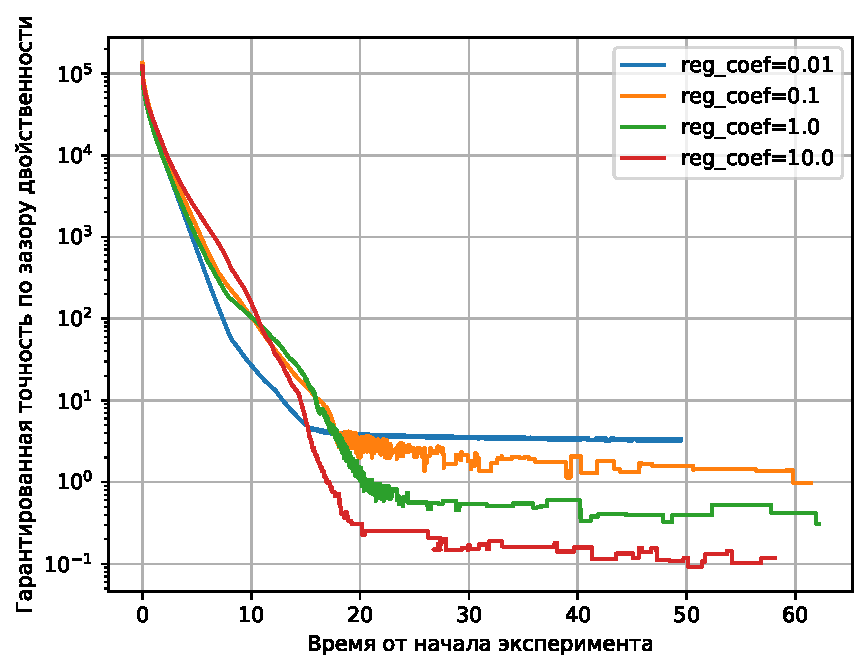
\includegraphics[width=.3\textwidth]{pics/3/subgradient/lasso_gap_vs_time_reg_coef.pdf}
 		} &

		\subfloat[градиентный метод]{
    		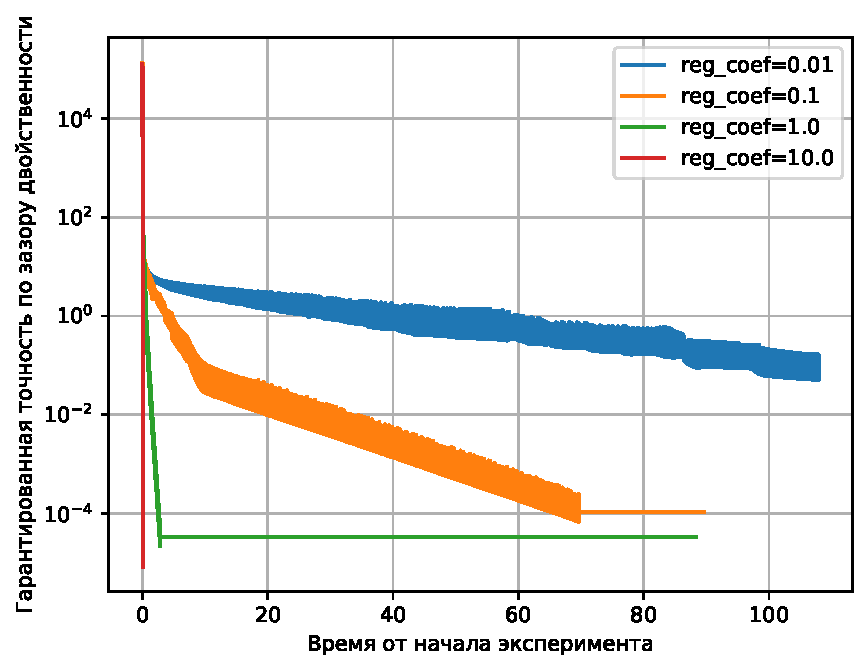
\includegraphics[width=.3\textwidth]{pics/3/proximal/lasso_gap_vs_time_reg_coef.pdf}
 		} &
 		
 		\subfloat[уск. градиентный метод]{
    		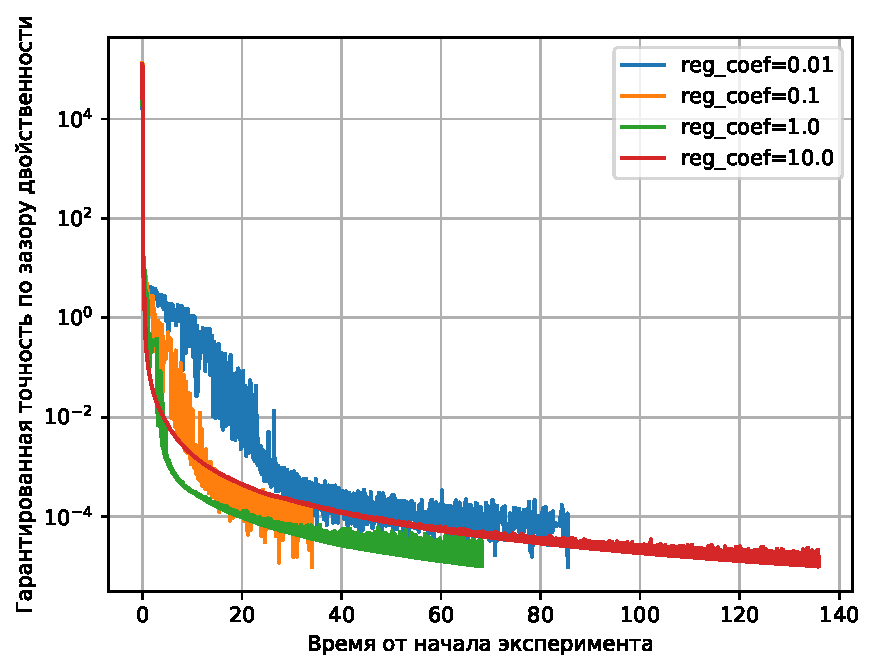
\includegraphics[width=.3\textwidth]{pics/3/proximal_fast/lasso_gap_vs_time_reg_coef.pdf}
 		}
   \end{tabular}
   \captionsetup{justification=centering}
   \caption{Гарантированная точность по зазору двойственности в зависимости от времени при разных $\lambda$ }
\end{figure}

Чем больше коэффициент регуляризации, тем быстрее методы достигают меньших значений зазора двойственности. Однако, для ускоренного метода не видно такой явной зависимости.
Стоит при этом заметить, что при всех значениях коэффициента регуляризации $\lambda$, кроме $\lambda=10$, ускоренный метод сошелся быстрее обычного градиентного метода.

\section{Выводы.}
В данной работе мы изучили субгрдиентный и градиентный методы. Рассмотрели, как они работают на разных данных, показали, что градиентный метод действительно делает примерно две внутренние итерации одномерного поиска и увидели, как влияют на работу субградиентного метода выбор начальной точки и длины начального шага.
\end{document}